\documentclass[twoside,english]{uiofysmaster}

\bibliography{references}
\usepackage{simplewick}
\usepackage{float}

% Adding nicer font to listings
\usepackage{ifxetex}
\ifxetex
  \usepackage{fontspec}
  \newfontfamily\listingsfontfamily[Scale=0.85]{Droid Sans Mono}
  \renewcommand{\listingsfont}{\listingsfontfamily}
\fi


\author{Fredrik Wilhelm Holmen}
\title{Master thesis Wilhelm Coupled Cluster}
\date{Autumn 2015}

\begin{document}
% set space around equations
\setlength{\belowdisplayskip}{12pt} \setlength{\belowdisplayshortskip}{12pt}
\setlength{\abovedisplayskip}{12pt} \setlength{\abovedisplayshortskip}{12pt}


\maketitle

\begin{abstract}
  This is an abstract text.
\end{abstract}

\begin{dedication}
  To someone
  \\\vspace{12pt}
  This is a dedication to my cat.
\end{dedication}

\begin{acknowledgements}
  I acknowledge my acknowledgements.
\end{acknowledgements}

\tableofcontents



\begin{chapter}{Introduction}
  This is a very nice introduction to my myster thesis.
  or ..
\end{chapter}





\begin{chapter}{Quantum Mechanics}
 	
	\begin{section}{Postulates}
 		Quantum mechanics is built upon by a few principles \cite{Audun,Griffiths,Sakurai,Susskind2014}, often called the postulates of quantum mechanics. 
 		\begin{enumerate}
 			\item \textbf{The Wave Function} \\
 			All information on a quantum system is given by the wave function $\left| \Psi(x,t) \right>$. The wave function represent the probability of measuring a particle within a small volume $\text{dx}$ and for a given time, $t$. As the probability cannot exceed $1$, the wave function must be normalized, namely
 			\begin{align}
 				\int_{-\infty}^\infty \Psi^*(x,t) \Psi(x,t) \text{dx} = 1
 			\end{align}
 			Physical distinguishable states are orthogonal to each other. Using normalized states, they are orthonormal to each other, meaning that for two unambigously distuingishable states, we have
 			\begin{align}
 				\left< \lambda | \psi \right> = \delta_{\lambda \psi}
 			\end{align}
 			\item \textbf{Observables}\\
			All observables are represented by linear operators, written with a "hat", $\hat O$. These linear operators are bound to be hermitian. An observable could also be called measurable quality. The outcome of a quantum mechanical experiment is an observable. 
			\item \textbf{Measurments}\\
			The possible outcomes of an experminent are the eigenvalues of an operator that represent the observable. Represented as a number $\lambda$. If a state is in the eigenstate $\left| \lambda \right>$, the only possible measurment of an experiment is the eigenvalue, $\lambda$. We write this as
 			\begin{align}
 				\hat O \left| \lambda \right> = \lambda \left| \lambda \right>
 			\end{align}
 			\item \textbf{Probabilities}\\
 			Given a state $\left| \alpha \right>$. The probability of observing $\lambda$ when measuring the observable $\hat O$ is given by 
 			\begin{align}
 				P(\lambda) = \left< \alpha | \lambda \right> \left< \lambda | \alpha \right> = | \left< \alpha | \lambda \right> |^2 
 			\end{align}
 			Which measures the overlap of the two states $\left| \alpha \right>$ and $\left| \lambda \right>$. If they are physically distinguishable, the probability is zero. If the probability is non-zero, we have "mixed states".
 			\item \textbf{Time development and the Schrodinger equation}\\
 			Time developement for states are given by acting on the state with a unitary operator
 			\begin{align}
 				\left| \Psi(t) \right> = \hat U(t) \left| \Psi(0) \right>
 			\end{align}
 			This leads us to the time-independent Schrodinger equation
 			\begin{align}
 				\hat H \left| \Psi(x,t) \right> = i \hbar \frac{\partial}{\partial t} \left| \Psi(x,t) \right> 
 			\end{align}
 			Where we have defined the Hamiltonian operator $\hat H$. The Hamiltonian will be used throughout the thesis, as its eigenvalues are the measurable energy. We will primerily be focused on solving the \textit{time independent} Schrodinger equation
 			\begin{align}
 				\hat H \left| \Psi(x) \right> = E \left| \Psi(x) \right> 
 			\end{align}
 		\end{enumerate}
 	\end{section}


 	\begin{section}{The Born-Oppenheimer Approximation}
 		The Born-Oppenheimer approximation lies at the heart of many-body quantum mechanics. 
 	\end{section}

 	\begin{section}{Pauli's Exclusion Principle}
 		Pauli exclusion principle, also called the antisymmetry principle \cite{Szabo} 
 	\end{section}

	\begin{section}{The Variational Principle}

	\end{section}

	\begin{section}{Slater Determinant}
		A system composed of a nuclei and electrons moving in accordance to the forces of electromagnetic attraction can be described by assigning each electron
		a wave function 
		\begin{align}
			\phi_i(\mathbf{x}_i)
		\end{align}
		Where $\mathbf{x}_i$ is the position vector for the electron i. Describing a system of many electrons can be done writing a Slater Determinant
		\begin{align}
			\ket{\Phi_0} = \frac{1}{ \sqrt{N!} } \left|\begin{matrix}
				\phi_1(\mathbf{x}_1) & \phi_2(\mathbf{x}_1) & ... & \phi_N(\mathbf{x}_1) \\
				\phi_1(\mathbf{x}_2) & \phi_2(\mathbf{x}_2) & ... & \phi_N(\mathbf{x}_2) \\
				... & & & \\
				\phi_1(\mathbf{x}_N) & \phi_2(\mathbf{x}_N) & ... & \phi_N(\mathbf{x}_N) 
			\end{matrix} \right|
		\end{align}
		This way of writing the many-body wave function will represent linear a combination of products of the one-body wave functions $\phi_i$'s and all the electronic coordinates
		$\mathbf{x}_i$ distributed among them in all possible ways. Exchanging two lines will change the sign such that the Slater Determinant will respect the anti-symmetry 
		requirement. \par
		We can choose the one-body wave functions that is most rewarding the specified system. When calculating on electrons moving with respect to a nuclei, one can choose the wave
		functions to be the 1s, 2s, 2p, .. orbitals. This representation will not, however, take into account the Colombic repulsion between two electrons and will only be an 
		approximation to the true wavefunction, $\ket{\Psi}$.
	\end{section}

	\begin{section}{Matrix Elements}
		
	\end{section}

\end{chapter}





\begin{chapter}{Second Quantization}
 	Second quantization is a new method of representing states and operators. 
	\begin{section}{Annihilation and Creation operators}
		We introduce a new way of writing states using the mathematical technique known as second quantization. The main goal is to treat states without paying attention
		to individual particle coordinates. We represent the empty space with the symbol for vacuum
		\begin{align}
			\ket{0}
		\end{align}
		To represent a state, we use a creation operator to add the state to the vacuum.
		\begin{align}
			\hat a_i^{\dagger} \ket{0} = \ket{\phi_i}
		\end{align}
		And the annihilation operator will remove the particle again. 
		\begin{align}
			\hat a_i \ket{\phi_i} = \ket{0}
		\end{align}
		Trying to add a new particle to an already filled state and removing an unoccupied state results in zero.
		\begin{align}
			\hat a_i^{\dagger} \ket{\phi_i} = 0 \;\;\;\;\; \hat a_i \ket{0} = 0
		\end{align}
		Bra states are needed, and by looking at the adjoint of a ket state, we get
		\begin{align}
			\left(\left| \phi_i \right> \right)^\dagger = \left< \phi_i \right| 
		\end{align}
		Which results in
		\begin{align}
			\left( \hat a_i^\dagger \left| 0 \right> \right)^\dagger = \left< 0 \right| \hat a_i = \left< \phi_i \right|
		\end{align}
		We see that the creation and annihilator operatorare each other's adjoint operator. We can define the counting operator, $\hat N$, which will count how many states are occupied in a Slater determinant
		\begin{align}
			\hat N = \sum_p \hat a^\dagger_p \hat a_p = \sum_p \hat n_p
		\end{align}
	\end{section}

	\begin{section}{Strings of Operators}
		We can now construct the Slater determinant by working on vacuum with a string of creation operators
		\begin{align}
			\hat a_1^{\dagger} \hat a_2^{\dagger}... \hat a_N^{\dagger} \ket{0} = \left| \phi_1 \phi_2 ... \phi_N \right>
		\end{align}
		Permutations of the operators introduces a sign-change, which is equivalent to interchanging rows in the determinant. We need second quantization to respect the anisymmetrization condition, so a permutation of two states should introduce a change of sign
		\begin{align}
			\hat a_1^{\dagger} \hat a_2^{\dagger} \ket{0} = \ket{\phi_1 \phi_2} = -\ket{\phi_2 \phi_1} = -\hat a_2^{\dagger} \hat a_1^{\dagger} \ket{0}
		\end{align}
		We introduce the permutation operator, $\hat P$, which permutes two states in the Slater determinant 
		\begin{align}
			\hat P \left| \Phi \right> = (-1)^{\sigma(P)} \left| \Phi \right>
		\end{align}
		Where $\sigma(P)$ counts how many times the states are interchanged. Demonstrated with creation operators
		\begin{align}
			\hat a_1^\dagger \hat a_2^\dagger ... \hat a_i^\dagger \hat a_j^\dagger ... \hat a_n^\dagger = - \hat a_1^\dagger \hat a_2^\dagger ... \hat a_j^\dagger \hat a_i^\dagger ... \hat a_n^\dagger
		\end{align}
	\end{section}

	\begin{section}{Anticommutator Relations}
		When working on strings of operators, it is very convenient to introduce anticommutator relations. We define the relation as 
		\begin{align}
			\{ \hat A, \hat B \} = \hat A \hat B + \hat B \hat A	
		\end{align}
		By inserting the annihilation and creation operator, we can compute the relations and look at how they work on the vacuum state 
		\begin{align}
			\{ \hat a_i^\dagger \hat a_j \} \left| 0 \right>  &= \hat a_i^\dagger \hat a_j \left| 0 \right>  + \hat a_j \hat a_i^\dagger \left| 0 \right> = 0 + \delta_{ij} \left|0\right> 
 		\end{align}
 		Where we have introduced the kroenecker-delta function
 		\begin{align}
 			\delta_{ij} = \begin{cases}
 						1, & \text{if } i = j \\
 						0, & \text{ij } i \neq j
 						\end{cases}
 		\end{align}
		The second case
		\begin{align}
			\{ \hat a_i \hat a_j^\dagger \} \left| 0 \right> &= \hat a_i \hat a_j^\dagger + \hat a_j^\dagger \hat a_i \left| 0 \right> = \delta_{ij} \left| 0 \right> + 0
		\end{align}
		And the two last cases
 		\begin{align}
			\{ \hat a_i \hat a_j \} \left| 0 \right> &= \hat a_i \hat a_j \left| 0 \right> + \hat a_j \hat a_i \left| 0 \right> = \hat a_i \hat a_j \left| 0 \right> - \hat a_i \hat a_j \left| 0 \right> = 0\\
			\{ \hat a_i^\dagger \hat a_j^\dagger \} \left| 0 \right> &= \hat a_i^\dagger \hat a_j^\dagger \left| 0 \right> + \hat a_j^\dagger \hat a_i^\dagger \left| 0 \right> = \hat a_i^\dagger \hat a_j^\dagger \left| 0 \right> - \hat a_i^\dagger \hat a_j^\dagger \left| 0 \right> = 0
 		\end{align}

 		Ending up with our relations
 		\begin{align}
 			&\{ \hat a_i \hat a_j \} = 0 \\
 			&\{ \hat a_i^\dagger \hat a_j^\dagger \} = 0 \\
			&\{ \hat a_i^\dagger \hat a_j \} = \{ \hat a_i \hat a_j^\dagger \} = \delta_{ij}
		\end{align}
		The last result is very useful for rewriting strings of operators, since it allows us to rewrite a set of two operators as
		\begin{align}
			\hat a_i^\dagger \hat a_j = \{ \hat a_i^\dagger \hat a_j \} - \hat a_j \hat a_i^\dagger = \delta_{ij} - \hat a_j \hat a_i^\dagger 
			\label{interchange operators}
		\end{align}
		Which will be at the center of Wick's theorem. 
	\end{section}

	\begin{section}{Inner products}
		We assume all states are orthonormal, taking the inner product of two states should give
		\begin{align}
			\left< i | j \right> = \delta_{ij}
		\end{align}
		And for consistency, the vacuum state must also be normalized
		\begin{align}
			\left< 0 | | 0 \right> = 1
		\end{align}
		this can be demonstrated by looking at the definition of the inner product of two equal states and using the anticommutator relations
		\begin{align}
			1 = \left< i | i \right> &= \left< 0 | \hat a_i \hat a_i^\dagger | 0 \right> \\
									 &= \left< 0 | (\delta_{ij} - \hat a_i^\dagger \hat a_i) | 0 \right> \\
									 &= \left< 0 | 0 \right> - 0 = \left< 0 | 0 \right>
		\end{align}
		It turns out we can use this exact scheme for longer chains of operators as well. Looking at the inner product of two general Slater Determinants
		\begin{align}
			&\left| A \right> = \left| a_1 a_2 ... a_N \right> = \hat a_1^\dagger \hat a_2^\dagger ... \hat a_N^\dagger \left| 0 \right> \\
			&\left| B \right> = \left| b_1 b_2 ... b_N \right> = \hat b_1^\dagger \hat b_2^\dagger ... \hat b_N^\dagger \left| 0 \right>
		\end{align}
		Writing the inner product
		\begin{align}
			\left< A | B \right> = \left< 0 | \hat a_N ... \hat a_2 \hat a_1 \hat b_1^\dagger \hat b_2^\dagger ... \hat b_N^\dagger | 0 \right>
		\end{align}
		By moving the annihilation operators all the way to the right, we know that the inner product becomes zero because $\hat a_p \left| 0 \right> = 0$. We utilize the anticommutator relations for interchanging creation and annihilation operators shown in (\ref{interchange operators}). By first moving $a_1$ to the right, we get two possible outcomes
		\begin{enumerate} 
			\item One $b_p$ is equal to $a_1$ and we get
			\begin{align}
				\hat a_1 \hat b_p^\dagger = \delta_{a_1,b_p} - \hat b_p^\dagger \hat a_1 = 1 - \hat b_p^\dagger \hat a_1 
				\label{InnerProduct1}
			\end{align}
			This will now give us a new and shorter inner product
			\begin{align}
				\left< A | B \right> = \left< 0 \right| \hat a_N ... \hat a_2 \hat b_1^\dagger... \hat b_{p-1}^\dagger \hat b_{p+1}^\dagger ... \hat b_N^\dagger \left| 0 \right>(-1)^{p-1} - \left< 0 \right| \hat a_N ... \hat a_2 \hat b_1^\dagger \hat b_2^\dagger ... \hat b_N^\dagger \hat a_1  \left| 0 \right>
			\end{align}
			Where the last term will vanish because of $\hat a_1 \left| 0 \right> = 0$. Notice the sign factor coming from $(-1)^{p-1}$. This is due to interchanging creation operators when moving $\hat b_p^\dagger$ from position $p$ and $(p-1)$ steps to the left before using (\ref{InnerProduct1}).  
			\item No $b_p$ is equal to $a_1$ and all $\delta_{a_1, b_p} = 0$. Applying the same logic as for outcome 1, we get
			\begin{align}
				\left< A | B \right> = 0
			\end{align}
		\end{enumerate}
		We do the same for all states and see that this inner product can only be non-zero if all states $a_1 .. a_N$ has a matching state in $b_1 .. b_N$ and vice versa. If the ordering of states is different, a permutation factor $-1^{\sigma(P)}$ is included. 
	\end{section}

	\begin{section}{Representation of Operators}
		Consider a symmetric one-body operator represented by
		\begin{align}
			\hat F = \sum_{\mu = 1}^N \hat f_\mu 
		\end{align}
		The number $\mu$ tells us on which particle $\hat F$ works on. In this case, we are looking at a symmetric operator because it works identically on all particles. Looking at a matrix element of $\hat F$ put petween two Slater determinants. 
		\begin{align}
			\left< a_1 a_2 ... a_N \right| \hat F \left| b_1 b_2 ... b_N \right> 
		\end{align}
		\begin{align}
			\sum_\mu \left< a_1 a_2 ... a_N \right| \hat f_\mu \left| b_1 b_2 ... b_N \right> 
		\end{align}

		\begin{subsection}{One-Body Operator}
			In second quantization, a one-body operator is given as
			\begin{align}
				\hat F = \sum_{pq} \left< p \right| \hat f \left| q \right> \hat a_p^\dagger \hat a_q 
			\end{align}
			Where the matrix element $\left< p \right| \hat f \left| q \right>$ is determined on the nature of the operator $\hat F$. It is common to denote this matrix element as
			\begin{align}
				\hat F = \sum_{pq} \left< p \right| \hat f \left| q \right> \hat a_p^\dagger \hat a_q = \sum_{pq} f_{pq} \hat a_p^\dagger \hat a_q
			\end{align}
			Doing calculations in many-body quantum mechanics, we are primerely interested in expectation values. It is therefore crucial that we develop a solid scheme for calculating these values. This can be done by for example looking at the following inner product 
			\begin{align}
				\left< P \right| \hat F \left| R \right> 
			\end{align}
			Inserting the definition of $\hat F$
			\begin{align}
				\left< 0 \right| \hat a_M ... \hat a_s \hat a_r \left( \sum_{kl} f_{kl} \hat a_k^\dagger \hat a_l \right) \hat a_p^\dagger \hat a_q^\dagger ... \hat a_N^\dagger \left| 0 \right>
			\end{align}
			Which can be rewritten as
			\begin{align}
				\sum_{pq} f_{pq} \left< 0 \right| \hat a_M ... \hat a_s \hat a_r (\hat a_k^\dagger \hat a_l) \hat a_p^\dagger \hat a_q^\dagger ... \hat a_N^\dagger \left| 0 \right>
			\end{align}
			We apply the same logic as in the previous section, which provides us with three different outcomes for this expectation value
			\begin{enumerate}
				\item The states $p,q,...,N$ are all identical to the states $r,s,...,M$. This results in
				\begin{align}
					\left< P \right| \hat F \left| R \right> = \sum_k^N f_{kk} (-1)^{\sigma(P)}
				\end{align}
				Where we have included a perturbation factor in case the ordering of states is different in the two states. 
				\item If all states except one from each Slater determinant are equal, we get a \textit{noncoincidence} \cite{ShavittAndBartlett}
				\begin{align}
					(p = r), \: (s = q), \: ..., \: (n \neq m), \: ..., \: (N = N)
				\end{align}
				we can rewrite the expectation value as
				\begin{align}
					\sum_{pq} f_{pq} \left< 0 \right| \hat a_M ... \hat a_s \hat a_r (\hat a_k^\dagger \hat a_l) \hat a_p^\dagger \hat a_q^\dagger ... \hat a_N^\dagger \left| 0 \right> = (-1)^{\sigma(P)} f_{mn}
				\end{align}
				Because the operators $\hat a_k^\dagger$ and $\hat a_l$ must be paired with the non-identical states $m$ and $n$ for us to be left with a orthogonal inner product.
				\item If there are more than one noncoincidence, no contributions can survive, and the expectation value is 
				\begin{align}
					\left< P \right| \hat F \left| R \right> = 0
				\end{align}
			\end{enumerate}
		\end{subsection}

		\begin{subsection}{Two-body Operator}
			I have in this thesis only looked at Hamiltonians consisting of a maximum of two-body interactions. Because of this, I will need a formalism for a two-body operator as well. It is defined almost identically as the one-body operator. We write the general two-body operator as
			\begin{align}
				\hat G = \frac{1}{2} \sum_{ijkl} \left< i(1) j(2) \right| g_{12} \left| k(1) l(2) \right> \hat a_i^\dagger \hat a_j^\dagger \hat a_l \hat a_k
			\end{align}
			Where the numbers $(1)$ and $(2)$ show which particle occupy the what state. We are, as for the one-body operator, interested in how we can calculate expectation values for this operator. We take the inner product with the SD's $\left| P \right>$ and $\left| R\right>$.
			\begin{align}
				\frac{1}{2} \sum_{ijkl} \left< i(1) j(2) \right| g_{12} \left| k(1) l(2) \right>   \left< 0 \right| \hat a_M ... \hat a_s \hat a_r (\hat a_i^\dagger \hat a_j^\dagger \hat a_l \hat a_k) \hat a_p^\dagger \hat a_q^\dagger ... \hat a_N^\dagger \left| 0 \right>
			\end{align}
			There are three possible outcomes here as well 
			\begin{enumerate}
				\item If there are none noncoincidences, and all states in SD $\left| P \right>$ is equal to all states in SD $\left| R \right>$, we get 
				\begin{align}
				 	\left< P \right| \hat G \left| R \right> = \frac{1}{2}\sum_{p \in P}\sum_{q \in P} (\left< pq\right| \hat g \left| pq \right> - \left< pq\right| \hat g \left| qp \right> ) = \frac{1}{2}\sum_{p \in P}\sum_{q \in P} \left< pq || pq \right>
				\end{align}
				Where it is useful to use the antisymmetric matrix element
				\begin{align}
					\left< pq || pq \right> = \left< pq\right| \hat g \left| pq \right> - \left< pq\right| \hat g \left| qp \right>  
				\end{align}
				\item If we have a single noncoincidence, where all states except one from each SD are perfectly identical, we get \cite{ShavittAndBartlett}
				\begin{align}
					\left< P \right| \hat G \left| R \right> = \sum_{q \in P} \left< p' q || p q \right>
				\end{align}
				where the states $p'$ and $p$ are the unequal states. 
				\item If we have two noncoincidences, we get 
				\begin{align}
					\left< P \right| \hat G \left| R \right> = \left< p' q' || p q \right> 
				\end{align}
				\item If more than two states from each SD are unequal, the expectation value will be $0$.
			\end{enumerate}
		\end{subsection}

		\begin{subsection}{The Hamiltonian}
			We can now write our Hamiltonian using second quantization. The Hamiltonian consist of a one-body and a two-body term
			\begin{align}
				\hat H = \hat H_1 + \hat H_2
			\end{align}
			Which can be written out as
			\begin{align}
				\hat H_1 = \sum_\mu \hat h_\mu, \:\;\;\;\;\; \hat H_2 = \sum_{\mu < \nu} \hat v_{\mu \nu}
			\end{align}
			Using atomic units, we can write this as
			\begin{align}
				\hat h_\mu = -\frac{1}{2}\nabla_\mu^2 - \sum_A \frac{Z_A}{r_{\mu A}}, \:\;\;\;\;\; \hat v_{\mu \nu} = \frac{1}{r_{\mu \nu}}
			\end{align}
			Using the formalism introduced, we can write this as
			\begin{align}
				\hat H = \hat H_1 + \hat H_2 = \sum_{ij} \left<i \right| \hat h \left| j \right> \hat a_i^\dagger \hat a_j 
						+ \frac{1}{4} \sum_{ijkl} \left<ij|| kl \right> \hat a_i^\dagger \hat a_j^\dagger \hat a_l \hat a_k
			\end{align}
			Where we have used the anti-symmetric form of the two-body operator
			\begin{align}
				\left<ij|| kl \right> = \left< i(1) j(2) \right| \hat v_{12} \left| k(1) l(2) \right> - \left< i(1) j(2) \right| \hat v_{12} \left| l(1) k(2) \right>
			\end{align}
		\end{subsection}

	\end{section}

	\begin{section}{Normal Ordering and Wick's Theorem}
		As one can see, calculations of inner products can be a tedious affair when utilizing the anitcommutator rules. Luckily, one can develop more powerful tools, namely Wick's theorem. Before introducing Wick's theorem, a definition of normal ordering and contractions are needed
		\begin{subsection}{Normal Ordering}
			As previously shown, when evaluating a string of operators, the general scheme is to place all annihilation operators to the right of creation operators. This is because, when working on the true vacuum state, annihilation operators give zero. The only non-zero results will then arize from kroenecker delta's when permutating creation-annihilation operators according to (\ref{interchange operators}). 

			A string of operators with all annihilation operators to the right will be referred to as a \textit{normal ordered} string of operators. Normal ordering of operators is commonly denoted by a curvy bracket or square bracket
			\begin{align}
				n[ \hat A \hat B ... \hat N ] = \{ \hat A \hat B ... \hat N \}
			\end{align}
			Any expectation value, with respect to the true vacuum, of a set of normal ordered operators will always be zero
			\begin{align}
				\left< 0 \right| \{ \hat A \hat B ... \hat N \} \left| 0 \right> = 0 
				\label{NormalOrdering1}
			\end{align}
			One can note that the Hamiltonian operator is already written in a \textit{normal ordered} form. 
		\end{subsection}

		\begin{subsection}{Contractions}
			The second tool needed for Wick's theorem is the definition \textit{contractions} of operators. We define the contraction of general creation and annihilation operators as
			\begin{align}
				\bcontraction{}{\hat A}{}{\hat B} 
				\hat A \hat B
				\equiv \hat A \hat B - \{ \hat A \hat B \}
			\end{align}
			Before taking the expactation value of the two operators with respect to the true vacuum. 
			Giving the results
			\begin{align}
				\bcontraction{}{\hat a_a^\dagger}{}{\hat a_b^\dagger}
				\hat a_a^\dagger \hat a_b^\dagger 
				= 
				\bcontraction{}{\hat a_a}{}{\hat a_b}
				\hat a_a \hat a_b
				= 
				\bcontraction{}{\hat a_a^\dagger}{}{\hat a_b}
				\hat a_a^\dagger \hat a_b
				= 0 
			\end{align}
			The only non-zero results will be for 
			\begin{align}
				\bcontraction{}{\hat a_a}{}{\hat a_b}
				\hat a_a \hat a_b
				^\dagger = \delta_{ab}
			\end{align}
		\end{subsection}
	
		\begin{subsection}{Time-independent Wick's theorem}
			Wick's theorem states: \textit{A product of a string of creation and annihilation operators is equal to their normal product plus the sum of all possible normal ordered contractions} \cite{ShavittAndBartlett}. Symbolically, this is shown by 
			\begin{align}
				\hat A \hat B \hat C \hat D ... = \{\hat A \hat B \hat C \hat D ... \} + \sum \{  \bcontraction[2ex]{}{\hat A}{\hat B \hat C \hat D ...}
				\hat A \bcontraction{}{\hat B}{\hat C \hat D ..}
				\hat B \hat C \hat D .... \}
			\end{align}
			The usefulness of this relation is when calculating expectation values. Because of (\ref{NormalOrdering1}), the only result that will give a non-zero result, is when all operators are fully contracted. As an example to display the usefulness of Wick's theorem 
			\begin{align}
				\left< 0 \right| \hat a_a \hat a_b^\dagger \hat a_c \hat a_d^\dagger \hat a_e \hat a_f^\dagger \left| 0 \right> = \left< 0 \right| \{ 
				\bcontraction{}{\hat a_a}{}{\hat a_b^\dagger}
				\hat a_a \hat a_b^\dagger \bcontraction{}{\hat a_c}{}{\hat a_d^\dagger}
				\hat a_c \hat a_d^\dagger \bcontraction{}{\hat a_e}{}{\hat a_f^\dagger}
				\hat a_e \hat a_f^\dagger 
				\} \left| 0 \right> = \delta_{ab} \delta_{cd} \delta_{ef}
			\end{align}
			Where the contractions displayed are the only set of non-zero contractions possible. 
		\end{subsection}
	\end{section}

	\begin{section}{Particle-Hole Formulation}
		For larger Slater determinants, it is tedious to write all states in terms of the vacuum state $\left| 0 \right>$. We define a reference state that will be used instead of the pure vacuum. Looking at a general Slater determinant
		\begin{align}
			\left| \Phi_0 \right> = \hat a_i^\dagger \hat a_j^\dagger ... \hat a_n^\dagger \left| 0 \right>
		\end{align}
		If this SD is the ground state of our system, we can use it as a reference state. We define the highest lying occupied state as the Fermi level, and name all states above the Fermi level \textit{particle states} or \textit{virtual states}. If a state below the Fermi level is vacant, we name it a \textit{hole state}. From here on out, we will use a distinct naming pattern for indices. Indices using the latin alphabet using letters $i, j, k, l, ...$ are reserved for \textit{hole states}. Latin letters $a, b, c, d, ...$ are reserved for \textit{particle states}. Sometimes, we want to name more general states that can take the form of either a \textit{hole state} or a \textit{particle state}. We use the latin letters $p, q, r, s, ...$. For a more convenient way of writing, operators will be written on a shorter and more convenient form
		\begin{align}
			\hat a_a = \hat a \:\:\:\:\: \hat a_b^\dagger = \hat b^\dagger \:\:\:\:\: \hat a_i^\dagger = \hat i^\dagger \:\:\:\: ...
		\end{align}
		And so forth. The reference state will be written as 
		\begin{align}
			\left| \Phi_0 \right> = \hat i^\dagger \hat j^\dagger \hat k^\dagger ... \hat n^\dagger \left| \right> = \left| ijk ... n \right> = \left| \right>
		\end{align}
		And excitations will be written as
		\begin{align}
			\text{Single Excitation: }\:\:\:\:& \left| \Phi_i^a \right> = \left| ajk ... n \right> = \hat i \hat a^\dagger \left| \right> \\
			\text{Double Excitation: }\:\:\:\:& \left| \Phi_{ij}^{ab} \right> = \left| abk ... n \right> = \hat i \hat j \hat a^\dagger \hat b^\dagger \left| \right> 
		\end{align}
		Where the use of annihilation operators for \textit{hole states} no longer produce zero when used on the reference state. But simply remove one particle from the reference state and create a \textit{hole state}. 
		\begin{align}
			\hat a_i \left| \right> = \left| \Phi_i \right> = \left| jk ... n \right>
		\end{align}
		This will introduce a small change in Wick's theorem, as the only non-zero contractions are now 
		\begin{align}
			\contraction{}{\hat i^\dagger}{}{\hat j}
			\hat i^\dagger \hat j = \delta_{ij}
		\end{align}
		And 
		\begin{align}
			\contraction{}{\hat a}{}{\hat b^\dagger}
			\hat a \hat b^\dagger = \delta_{ab}
		\end{align}
		Contractions relative to the Fermi vacuum will now be denoted by brackets \textit{above} the operators instead of below. Apart from this, Wick's theorem is unchanged relative to the Fermi vacuum. \par 


		A very important property of the reference state, is the expectation value for the hamiltonian. 
		\begin{align}
			\left< \right| \hat H \left| \right> = \left< \Phi_0 \right| \hat H \left| \Phi_0 \right> = \left< ijk...n \right| \hat H \left| ijk...n\right> 
		\end{align}
		We name this the reference Energy. The result is given by \cite{ShavittAndBartlett}
		\begin{align}
			E_{\text{ref}} = \left< \Phi_0 \right| \hat H \left| \Phi_0 \right> = \sum_i h_{ii} + \frac{1}{2} \sum_{ij} \left< ij || ij \right>
		\end{align}

	\end{section}

	\begin{section}{Normal ordering of Operators}
		After defining the new vacuum, we will now rewrite the operators with respect to the reference state.	
		\begin{subsection}{One-Body Operator}
			 Consider a general one-body operator
			\begin{align}
				\hat F = \sum_{pq} \left< p \right| \hat f \left| q \right> \hat p^\dagger \hat q
			\end{align}
			Using Wick's theorem to rewrite the string of operators
			\begin{align}
				\hat p^\dagger \hat q = \{\hat p^\dagger \hat q \} + \contraction{}{\hat p}{^\dagger}{\hat q}
				\hat p^\dagger \hat q
			\end{align}
			We get 	
			\begin{align}
				\hat F &= \sum_{pq} \left< p \right| \hat f \left| q \right> \{ \hat p^\dagger \hat q \} + \sum_i \left< i \right| \hat f \left| i \right>\\
					&= \hat F_N + \sum_i \left< i \right| \hat f \left| j \right>
			\end{align}
			We notice that since 
			\begin{align}
				\left< \right. | \hat F_N |\left. \right> = 0 \:\:\:\: \rightarrow \:\:\:\: \sum_i \left< i \right| \hat f \left| i \right> = \left< \right. | \hat F | \left. \right>
			\end{align}
			So we can rewrite the equation as
			\begin{align}
				\hat F = F_N + \left< \right. | \hat F | \left. \right>
			\end{align}
			Meaning that $F_N$ represent the difference between $\hat F$ and the Fermi expectation value. 
		\end{subsection}
		
		\begin{subsection}{Two-Body operators}
			The general two-body operator given by
			\begin{align}
				\hat G = \frac{1}{4} \sum_{pqrs} \left< pq | \hat g | rs \right>_A \hat p^\dagger \hat q^\dagger \hat s \hat r
			\end{align}
			Although the method will be identical for a two-body operator as for a one-body operator, we will require a much larger sum over all possible contractions when using Wick's theorem. Calculation of the result can be viewed in \cite{ShavittAndBartlett}. 
			\begin{align}
				\hat G = \frac{1}{4} \sum_{pqrs} \left<pq | \hat g | rs\right>_A \{ \hat p^\dagger \hat q^\dagger \hat s \hat r \}+ \sum_{ipq} \left<pi |\hat g | qi\right>_A \{ \hat p^\dagger \hat q\} + \frac{1}{2} \sum_{ij} \left< ij | \hat g | ij \right>_A 
				\label{Two-Body Normal Ordering}
			\end{align}
			As for the one-body operator
			\begin{align}
				\left< \right. | \hat G | \left.  \right> = \frac{1}{2} \sum_{ij} \left< ij | \hat g | ij \right>_A 
			\end{align}
			We can now name the terms 
			\begin{align}
				\hat G = \hat G_N + \hat G_N' + \left< \right. | \hat G | \left.  \right>
			\end{align}
			Where $\hat G_N'$ is a normal-ordered two-body operator. 

		\end{subsection}
	\end{section}

	\begin{section}{Partitioning the Hamiltonian Operator}
		The Hamiltonian has been shown to consist of a one-body and a two-body term
		\begin{align}
			\hat H = \hat H_1 + \hat H_2
		\end{align}
		One can, however, write it in terms of a zero-order term and a perturbation
		\begin{align}
			\hat H = \hat H_0 + \hat V
		\end{align}
		It is convenient to choose a zero-order Hamiltonian that is diagonal
		\begin{align}
			\hat H_0 = \sum_p \epsilon_p \hat p^\dagger \hat p
		\end{align}
		This means we can write the perturbation as
		\begin{align}
			\hat V &= (\hat H_1 - \hat H_0) + \hat H_2 \\
			&= \sum_{pq}(h_{pq} - \epsilon_p \delta_{pq} ) \hat p^\dagger \hat q + \frac{1}{4}\left<pq||rs\right>\hat p^\dagger \hat q^\dagger \hat s \hat r 
		\end{align}
		First, we define a Fock operator, $\hat F$, and a common practice is to choose the orbital energies as the diagonal elements of this Fock operator. 
		\begin{align}
			\hat F = \sum_{pq} f_{pq} \hat p^\dagger \hat q
		\end{align}
		With the matrix element defined as
		\begin{align}
			f_{pq} = h_{pq} + u_{pq}
		\end{align}
		here $u_{pq}$ is the matrix element of a one-body operator $\hat U$ implemented to simplify the zeroth-order term $\hat H_0$ and by simplifying the result when normal ordering the Hamiltonian later. See (\ref{Total Perturbation})
		\begin{align}
			\hat U &= \sum_{pq} u_{pq} \hat p^\dagger \hat q \\
			u_{pq} &= \sum_i \left<pi||qi\right>
		\end{align}
		This means we can write $\hat F = \hat H_1 + \hat U$. Inserting the Fock operator into the perturbation
		\begin{align}
			\hat V &= \hat F - \hat H_0 - \hat U + \hat H_2 \\
				   &= \sum_{pq}(f_{pq} - \epsilon_p \delta_{pq} - u_{pq}) \hat p^\dagger \hat q + \frac{1}{4} \sum_{pqrs} \left<pq||rs\right> \hat p^\dagger \hat q^\dagger \hat s \hat r
			\label{3.93}	
		\end{align}
		For a non-canonical Hartree-Fock case, the Fock matrix is diagonal, namely
		\begin{align}
			f_{pq} = \epsilon_p \delta_{pq}
		\end{align}
		This means the perturbation can be rewritten as
		\begin{align}
			\hat V = -\sum_{pq} u_{pq} \hat p^\dagger \hat q + \frac{1}{4} \sum_{pqrs} \left<pq||rs\right> \hat p^\dagger \hat q^\dagger \hat s \hat r	
			\label{3.95}
		\end{align}
		With the zeroth-order energies given by 
		\begin{align}
			\hat H_0 = \sum_p \epsilon_p \hat p^\dagger \hat p \;\;\;\;\;\; \epsilon_p = h_{pp} + \sum_i \left<pi||pi\right>
		\end{align}
		The noncanonical case, the Fock operator, $\hat F$, is block diagonal, with $f_{ia} = 0$. To, again, cancel out the single orbital energies from the perturbation, we split the Fock operator into a diagonal and off-diagonal term
		\begin{align}
			\hat F = \hat F^d + \hat F^o
		\end{align}
		The diagonal term will now be canceled out, and we are left with the perturbation
		\begin{align}
			\hat V = -\sum_{pq} (f_{pq}^o - u_{pq}) \hat p^\dagger \hat q + \frac{1}{4} \sum_{pqrs} \left<pq||rs\right> \hat p^\dagger \hat q^\dagger \hat s \hat r
		\end{align}
		For convience, we can organize the perturbation into a one-body part and a two-body part, $\hat V_1$ and $\hat V_2$
		\begin{align}
			\hat V_1 &= \hat F^o - \hat U = \sum_{pq} (f_{pq}^o - u_{pq}) \hat p^\dagger \hat q \\
			\hat V_2 &= \hat H_2 = \frac{1}{4} \sum_{pqrs} \left< pq||rs\right> \hat p^\dagger \hat q^\dagger \hat s \hat r
			\label{Partitioned Hamiltonian}
		\end{align}
		Resulting in the Hamiltonian
		\begin{align}
			\hat H = \hat H_0 + \hat V_1 + \hat V_2
		\end{align}

	\end{section}

	\begin{section}{Normal Ordering of Hamiltonian}
		To sum it all up, I will now present a normal ordering of the partitioned Hamiltonian operator. Starting by applying Wick's theorem to the zeroth order term
		\begin{align}
			(\hat H_0)_N = \hat H_0 - E^{(0)} = \sum_p \epsilon_p \hat p^\dagger \hat p - \sum_i e_i = \sum_p \epsilon_p \{\hat p^\dagger \hat p\}
		\end{align}
		Then applying Wick's theorem to the one- and two-body perturbations given in (\ref{Partitioned Hamiltonian})
		\begin{align}
			\hat V_1 = (\hat V_1)_N + \left< \right. | \hat V_1 | \left. \right>
		\end{align}
		Where we have 
		\begin{align}
			(\hat V_1)_N = \hat F_N^o - \hat U_N = \sum_{pq}(f_{pq}^o - u_{pq})\{ \hat p^\dagger \hat q \}
		\end{align}
		and
		\begin{align}
			\left< \right. | \hat V_1 | \left. \right> = -\sum_{ij} \left< ij || ij \right> = - \left< \right. | \hat U | \left. \right> 
		\end{align}
		Turning to the two-body perturbation and using (\ref{Two-Body Normal Ordering})
		\begin{align}
			\hat V_2 = (\hat V_2)_N + \hat V_N' + \left< \right. | \hat V_2 | \left. \right>
		\end{align}
		Where we have the following 
		\begin{align}
			(\hat V_2)_N &= \frac{1}{4} \sum_{pqrs} \left<pq||rs\right> \{ \hat p^\dagger \hat q^\dagger \hat s \hat r \} \\
			V_N' &= \sum_{pq} \left<pi||pi\right> \{ \hat p^\dagger \hat q \} \\
			\left< \right. | \hat V_2 | \left. \right> &= \frac{1}{2} \sum_{ij} \left<ij||ij\right>
		\end{align}
		We notice now, that after normal ordering the operators, we are left with many terms that can be reorganized into zero-, one- and two-body parts. We can rewrite the total perturbation as
		\begin{align}
			\hat V = \hat F_N^o - \hat U_N + \left< \right. | \hat V_1 | \left. \right> + (\hat V_2)_N + \hat V_N' + \left< \right. | \hat V_2 | \left. \right>
			\label{Total Perturbation}
		\end{align}
		Now, by construction of $\hat U$, we see that $\hat U$ and $\hat V_N'$ cancel each other out. Renaming $(\hat V_2)_N = \hat W_N$ We see that the terms left can be written as 
		\begin{align}
			\hat V = \hat F_N^o + \hat W_N + \left< \right. | \hat V | \left. \right>
		\end{align}
		By applying the same logic as earlier, we write
		\begin{align}
			\hat V_N = \hat V - \left< \right. | \hat V | \left. \right>
		\end{align}
		So that we finally can write the normal ordered perturbation as
		\begin{align}
			\hat V_N = \hat F_N^o + \hat W_N
		\end{align}
		We notice here the use of the diagonal Fock matrix. This matrix is just zero in the canonical Hartree Fock case. 
	\end{section}

	\begin{section}{Correlation Energy}
		All the many-body quantum mechanics methods described in this thesis will aim to compute the correlation energy. We derive it by substracting 
		\begin{align}
			\left< \right. | \hat H | \left. \right> = \left< \right. | \hat H_0 | \left. \right> + \left< \right. | \hat V | \left. \right>
		\end{align}
		from the partitioned hamiltonian $\hat H = \hat H_0 + \hat V$. Resulting in
		\begin{align}
			\hat H - \left< \right. | \hat H | \left. \right> &= \hat H_0 - \left< \right. | \hat H_0 | \left. \right> + \hat V - \left< \right. |\hat V| \left. \right>
		\end{align}
		This can be rewritten in terms of normal ordered operators as 
		\begin{align}
			\hat H_N = (\hat H_0)_N + \hat V_N
		\end{align}
		The Schrödinger equation for this operator is given as
		\begin{align}
			\hat H_N \Psi = \Delta E \Psi 
		\end{align}
		Where we have defined the computed energy as
		\begin{align}
			\Delta E = E - E_{\text{ref}}
		\end{align}
		or 
		\begin{align}
			E = E_{\text{ref}} + \Delta E
		\end{align}
		This energy is named the correlation energy, and the goal of my thesis has been to implement and compare different methods to compute this energy for different systems. The reference energy, given as
		\begin{align}
			E_{\text{ref}} = \left< \right. | \hat H_0 | \left. \right> + \left< \right. | \hat V | \left. \right>
		\end{align}
		Is easily computed when the basis is set up. Finally, we can set up the fully partitioned normal ordered Hamiltonian as
		\begin{align}
			\hat H_N = \hat F_N^d + \hat F_N^o + \hat W_N
		\end{align}

	\end{section}
 
\end{chapter}



\begin{chapter}{Diagramatic Representation}
	It can be quite cumbersome and error-prone to treat the manipulation of states and operators with second quantization \cite{ShavittAndBartlett}. The soon to be introduced many body methods will include various sums over states. One can introduce a new formalism originated in quantum field theory in the form of Feynman diagrams to depict and list these sums. It is quite common to refer to these sums simply as \textit{diagrams}. The main benefits of the diagramatic notation include an easy way of listing non vanishing terms and elucidating various cancelations in the sums. 

	\begin{section}{The Slater Determinant}
		We begin, as in second quantization, by setting up the Slater determinant. There is a time dependent direction on the diagrams going up. The actual times are irrelevant, but the sequence is important. The reference state, $| \left. \right> = \left| \Phi \right>$ is depicted simply as a horizontal line
		\begin{figure}[H]
		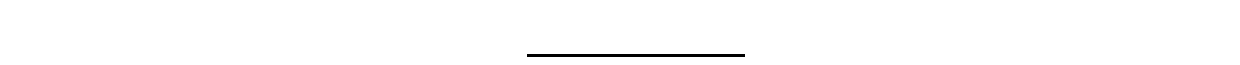
\includegraphics[width=\textwidth]{Figures/SlaterDeterminant1.pdf}
		\label{SlaterDeterminant1}
		\caption{Diagram for the reference state $| \left. \right>$}
		\end{figure}
		While the hole states are represented by vertical lines either going up or down, particle and hole states are depicted by a vertical line. An arrow pointing up relates a particle state, while an arrow pointing down will mean a hole state. Depicting the two states $\left| \Phi^a \right> $ and $\left| \Phi_i \right>$
		\begin{figure}[H]
			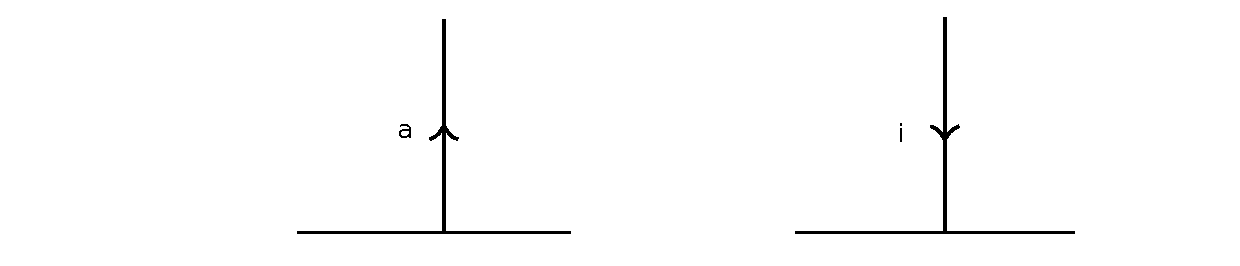
\includegraphics[width=\textwidth]{Figures/SlaterDeterminant2.pdf}
			\label{SlaterDeterminant2}
			\caption{Diagrams for the addition of a particle and a hole state, $\left| \Phi^a \right> $ and $\left| \Phi_i \right> $ respectively}
		\end{figure}
		The ket-variant of the singly excited Slater determinant $\left< \Phi_i^a \right| $ can be drawn as
		\begin{figure}[H]
			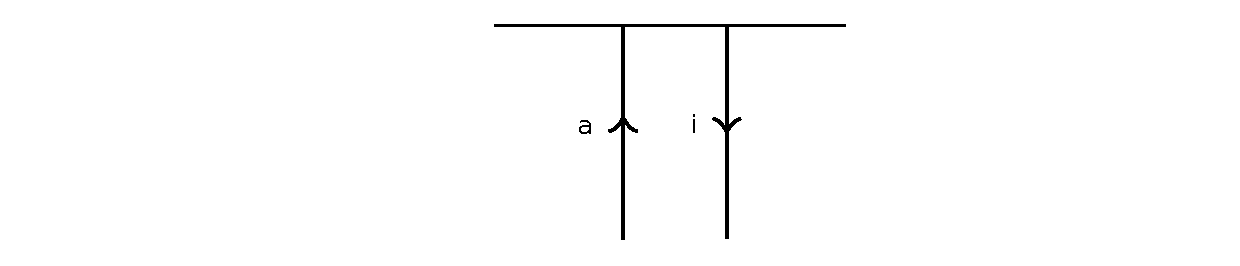
\includegraphics[width=\textwidth]{Figures/SlaterDeterminant3.pdf}
			\label{SlaterDeterminant3}
			\caption{Diagram for the singly excited ket state $\left< \Phi_i^a \right|$}
		\end{figure}
		And the doubly excited states $\left| \Phi_{ij}^{ab} \right>$ can be drawn as
		\begin{figure}[H]
			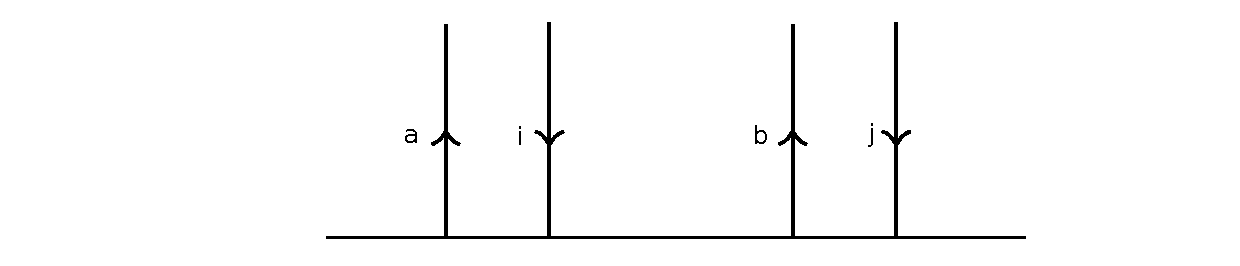
\includegraphics[width=\textwidth]{Figures/SlaterDeterminant4.pdf}
			\label{SlaterDeterminant4}
			\caption{Diagram for the doubly excited bra state $\left| \Phi_{ij}^{ab} \right>$}
		\end{figure}
	\end{section}

	\begin{section}{Operators}
		We need a convention for one body operators as well. The one body Hamiltonian operator is given by 
		\begin{align}
			\hat H_1 = \sum_{pq} \left< p | h | \right> \hat p^\dagger \hat q
		\end{align}
		We will represent the matrix element $\left< p | h | \right>$ by a dashed line, while there will be one line entering and one line leaving the operator due to the annihilation and creation operator. Because the operator behaves different depending on wether the general operators $p$ and $q$ are hole or particle states, the one body operator will I list the four normal ordered one body operators below \cite{ShavittAndBartlett}
		\begin{figure}[H]
			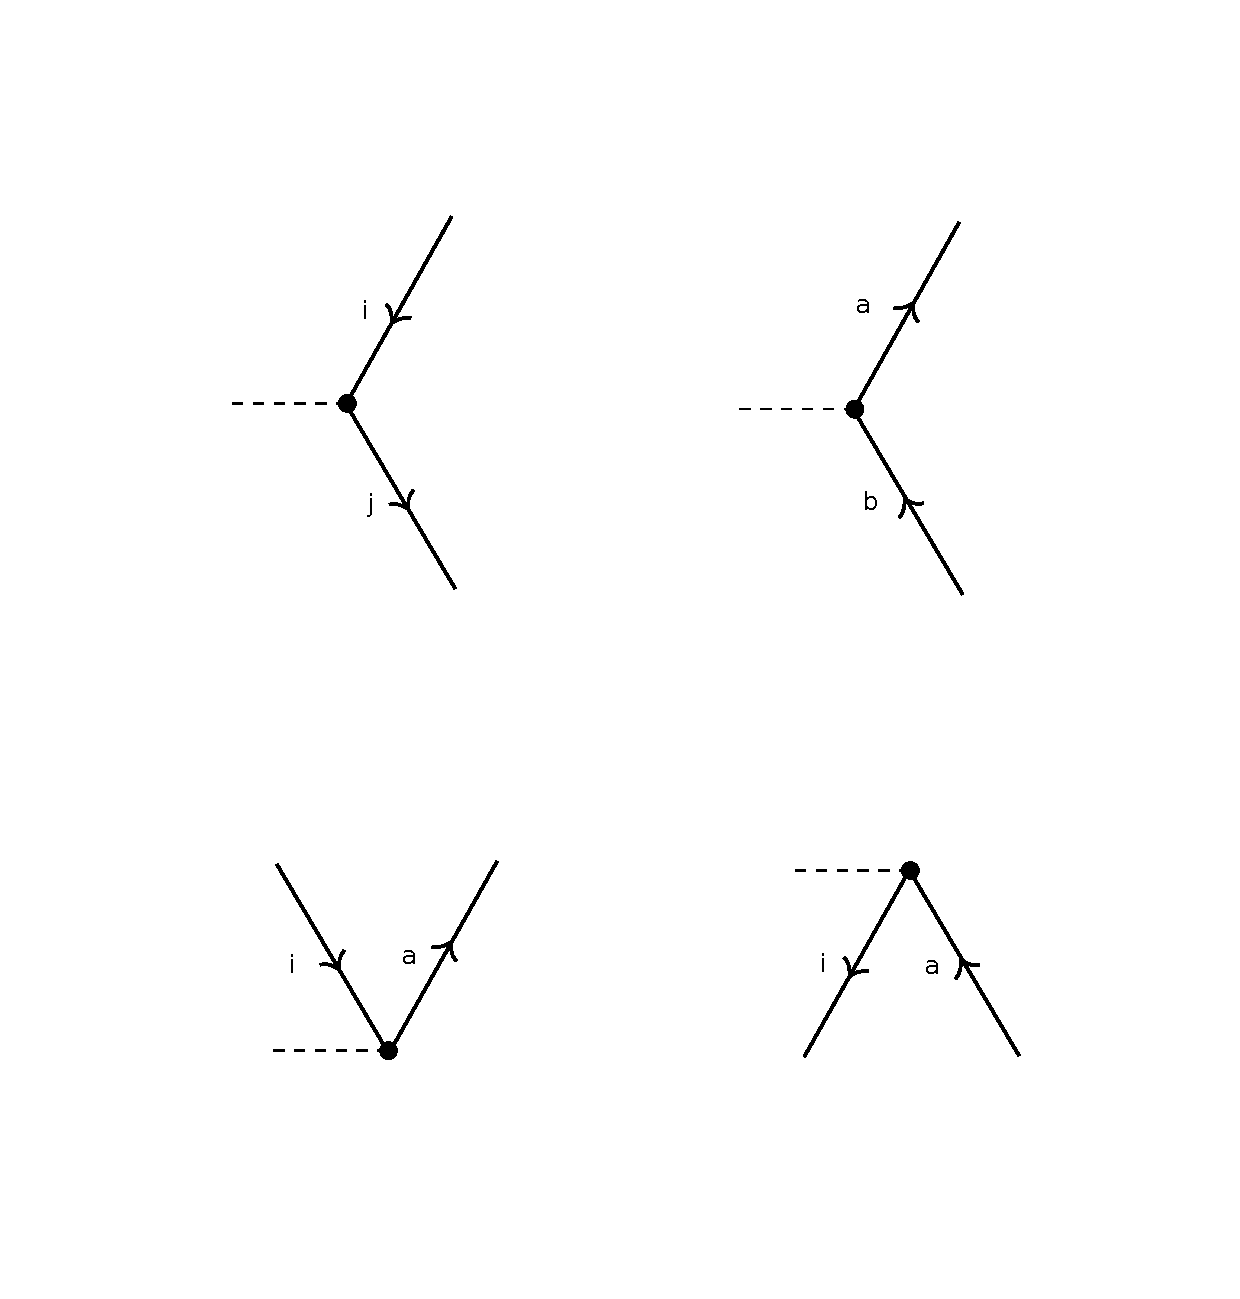
\includegraphics[width=\textwidth]{Figures/OneBodyOperator.pdf}
			\label{OneBodyOperator}
			\caption{Diagrams for four different variants of the one body operator. From left to right, the operators shown are $\sum_{ij} h_{ij} i^\dagger j $, $\sum_{ab} h_{ab} a^\dagger b$, $\sum_{ai}h_{ai} a^\dagger i$ and $\sum_{ai} h_{ia} i^\dagger a$}
		\end{figure}

		\begin{figure}[H]
			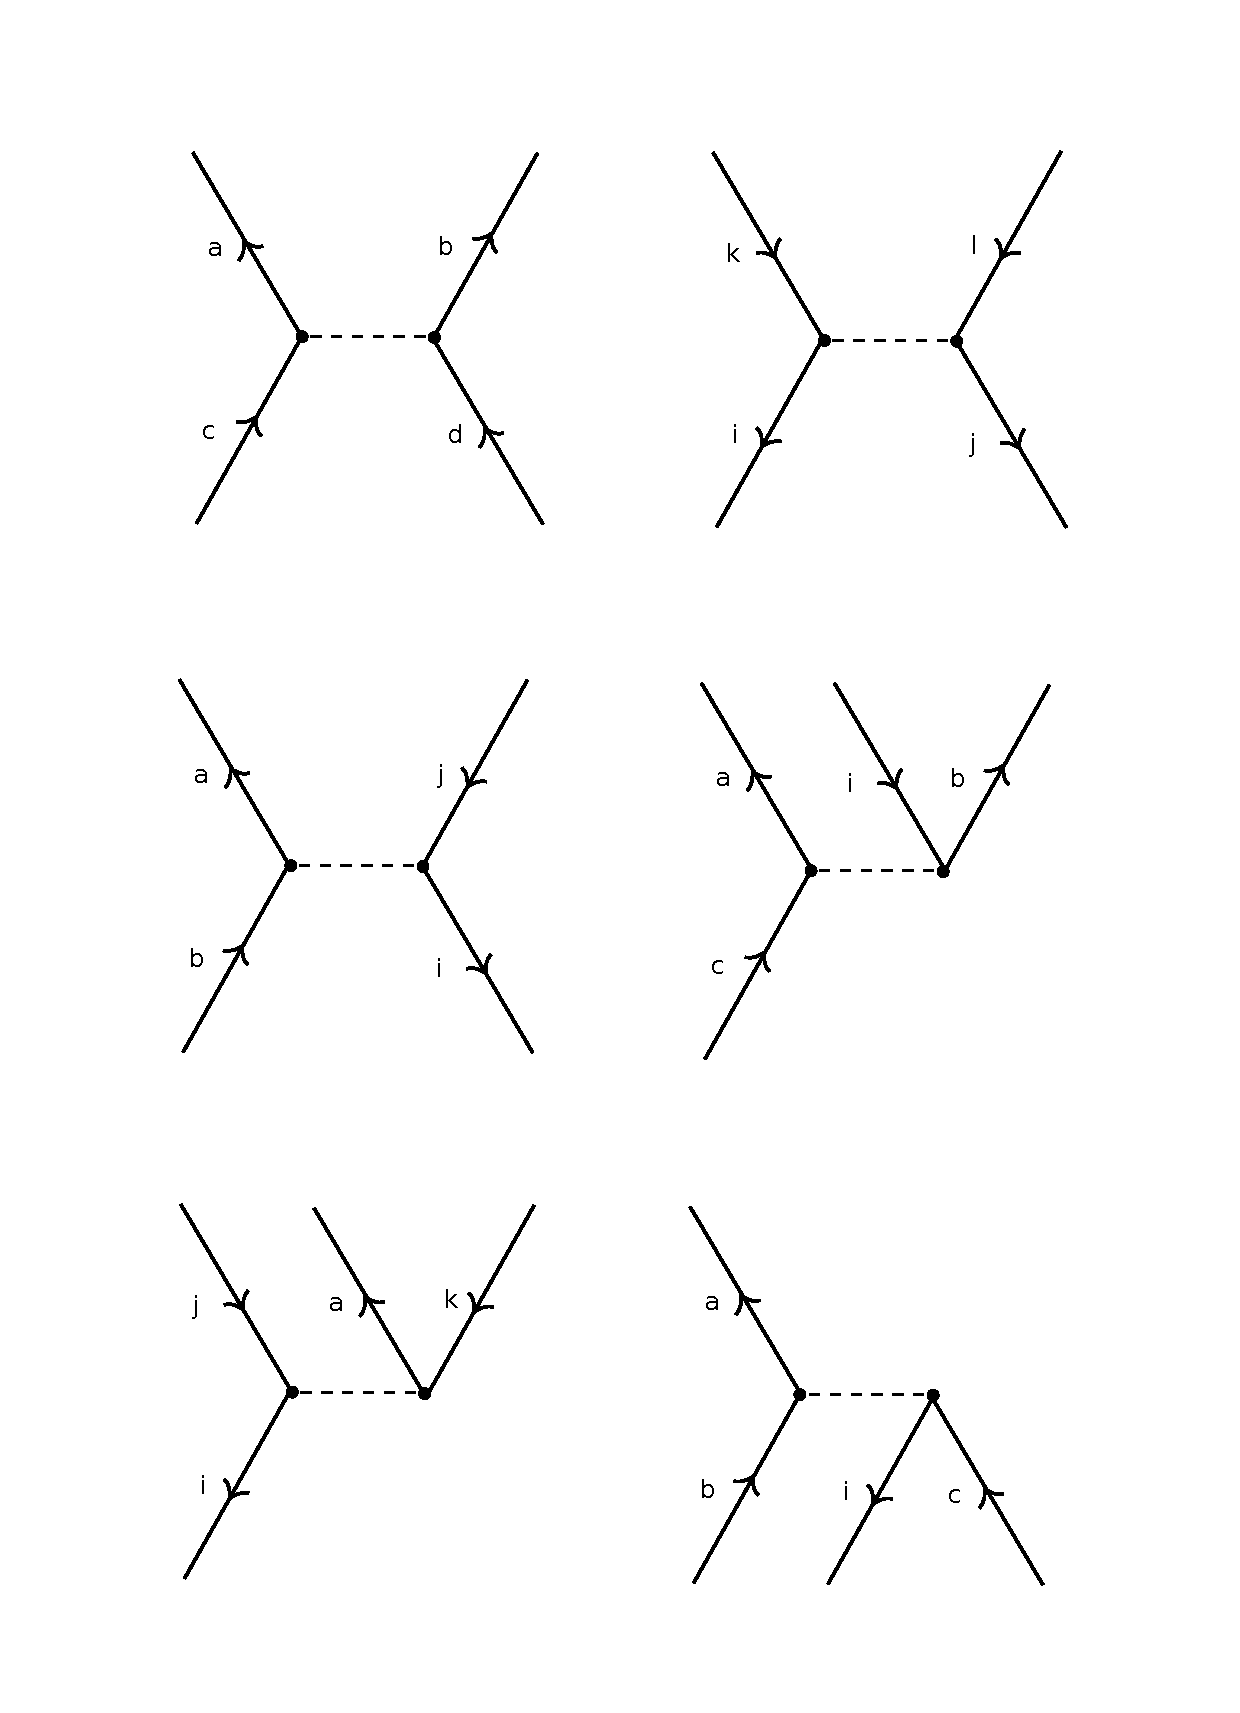
\includegraphics[width=\textwidth]{Figures/TwoBodyOperator.pdf}
			\label{TwoBodyOperator}
			\caption{Diagrams for four different variants of the one body operator. From left to right, the operators shown are $\sum_{ij} h_{ij} i^\dagger j $, $\sum_{ab} h_{ab} a^\dagger b$, $\sum_{ai}h_{ai} a^\dagger i$ and $\sum_{ai} h_{ia} i^\dagger a$}
		\end{figure}

		\begin{figure}[H]
			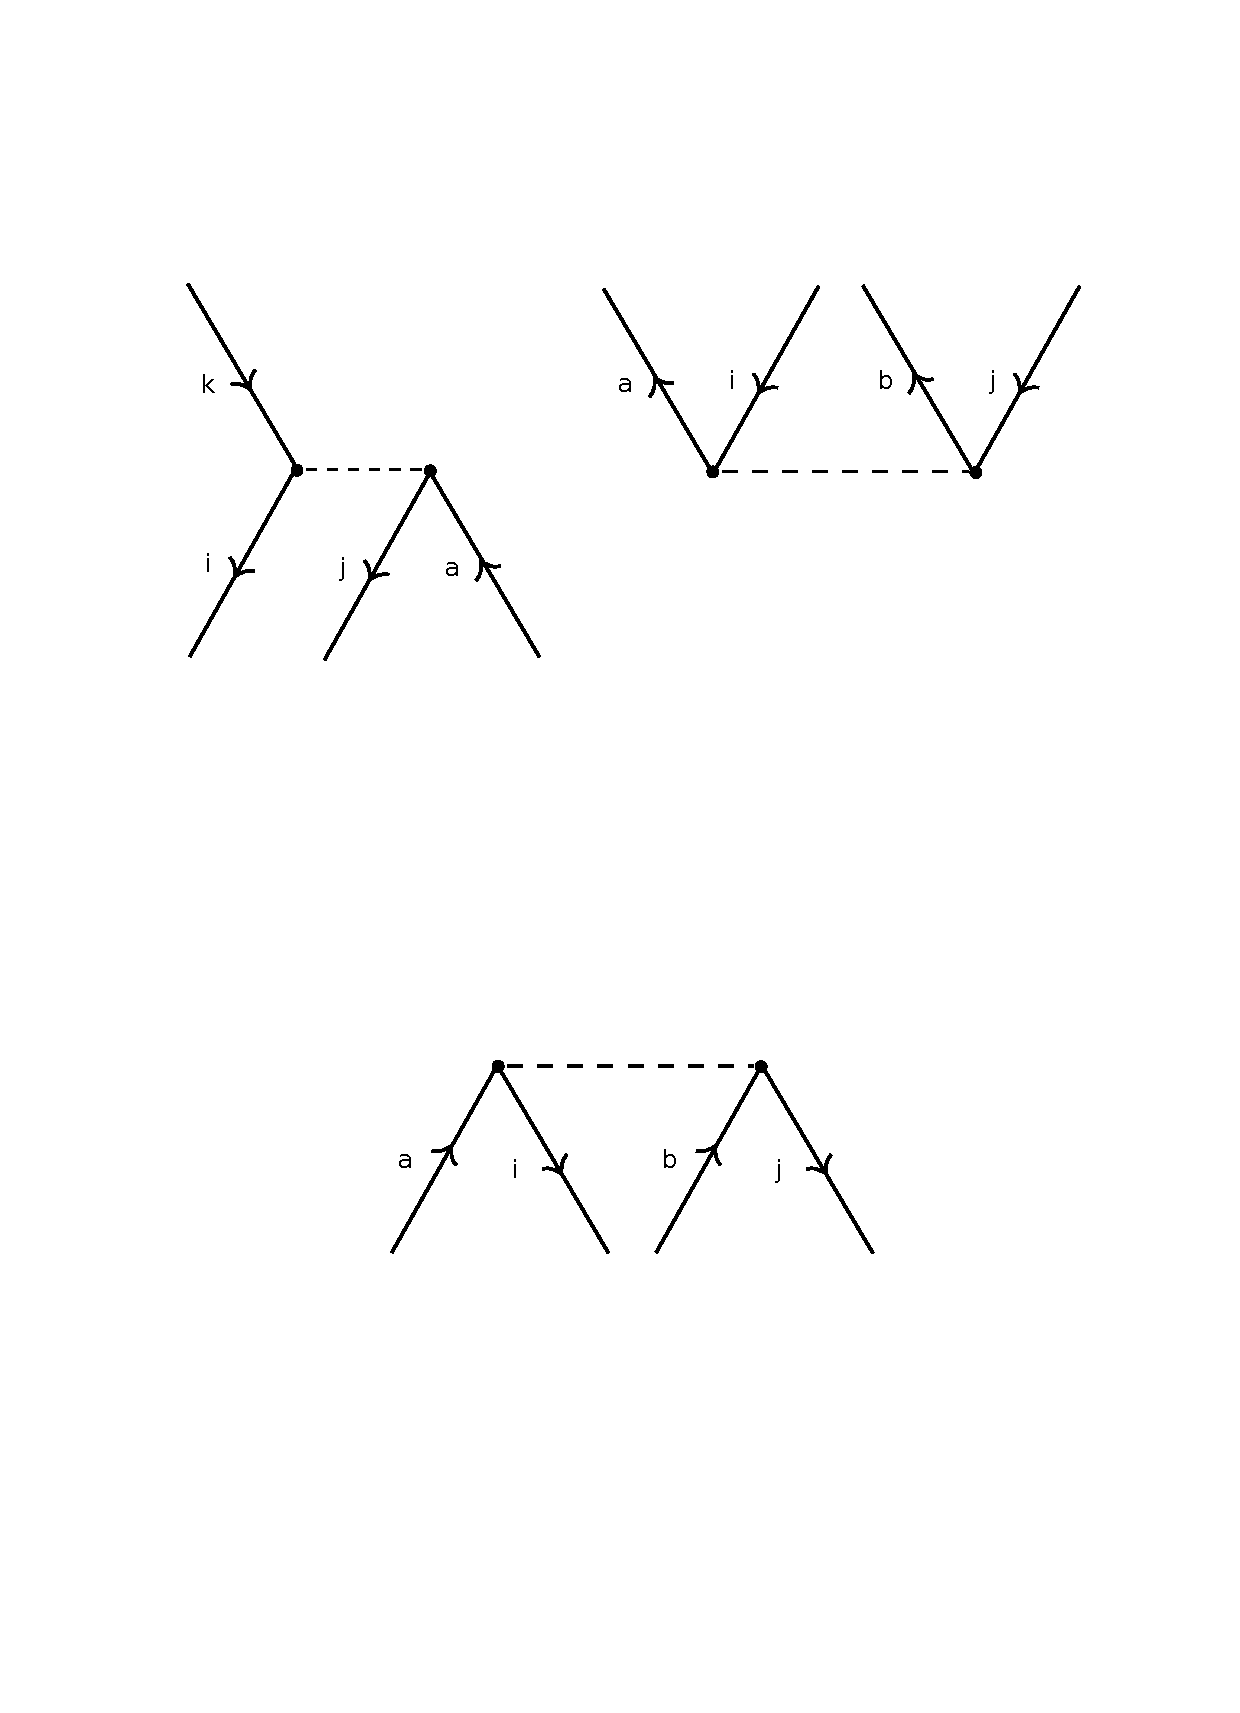
\includegraphics[width=\textwidth]{Figures/TwoBodyOperator2.pdf}
			\label{TwoBodyOperator2}
			\caption{Diagrams for four different variants of the one body operator. From left to right, the operators shown are $\sum_{ij} h_{ij} i^\dagger j $, $\sum_{ab} h_{ab} a^\dagger b$, $\sum_{ai}h_{ai} a^\dagger i$ and $\sum_{ai} h_{ia} i^\dagger a$}
		\end{figure}

	\end{section}

	\begin{section}{Contractions}
		
	\end{section}
	


\end{chapter}



\begin{chapter}{Many-Body Methods}
	We define an ansatz for the ground state, $\left| \Phi_0 \right>$ as a Slater determinant consisting of the single particle states, $\left| \phi_i \right>$
	\begin{align}
		\ket{\Psi} \approx \ket{\Phi_0} = 	\frac{1}{ \sqrt{N!} } \left|\begin{matrix}
			\phi_1(\mathbf{x}_1) & \phi_2(\mathbf{x}_1) & ... & \phi_N(\mathbf{x}_1) \\
			\phi_1(\mathbf{x}_2) & \phi_2(\mathbf{x}_2) & ... & \phi_N(\mathbf{x}_2) \\
			... & & & \\
			\phi_1(\mathbf{x}_N) & \phi_2(\mathbf{x}_N) & ... & \phi_N(\mathbf{x}_N) 
		\end{matrix} \right|
	\end{align}
	Written in terms of second quantization
	\begin{align}
		\left| \Phi_0 \right> = \left( \prod_{i \leq F} \hat i^\dagger \right) \left| 0 \right> = |\left.  \right> 
	\end{align}
	Typically one chooses well-known and mathematically simple single particle states that are easy to implement. In this thesis, I have used a free particle wave function as single-particle states for infinite matter. Using this basis, I obviously fail to incorporate the interaction between electrons since $\phi_1$ remains unchanged if I also add $\phi_2$. This can be solved by using a smarter basis, which is the goal of Hartree-Fock. Hartree-Fock will, through an iterative method, change the single particle states to get a better result. This can be viewed as incorporating the interaction as a \textit{mean field} approximation. 

	I will in this thesis present, and use, three \textit{post Hartree-Fock} methods. These are \textit{Full Configuration Interaction Theory}, \textit{Many Body Perturbation Theory} and \textit{Coupled Cluster Theory}, where the latter is the main focus of my thesis. These methods aim to compute the \textit{Corrolation Energy} as presented in the chapter on Second Quantization. It is quite common to first implement the Hartree-Fock method, providing the most precise reference energy. 

	\begin{section}{Full Configuration Interaction Theory}
		The first \textit{Post Hartree-Fock} method to be presented is the \textit{Full Configuration Interaction theory}. We expand the true wave function as a linear combination of the ground state ansatz and all possible excitations
		\begin{align}
			\left| \Psi \right> = C_0 \left| \Phi_0 \right> + \sum_{ai} C_i^a \left| \Phi_i^a \right> + \sum_{abij} C_{ij}^{ab} \left| \Phi_{ij}^{ab} \right> + ... 
		\end{align}
		Which can be rewritten in terms of a \textit{correlation operator}
		\begin{align}
			\left| \Psi \right> = ( C_0 + \hat C) \left| \Phi_0 \right> 
		\end{align}
		With
		\begin{align}
			\hat C = \sum_{ai} C_i^a \hat a^\dagger \hat i + \sum_{abij} C_{ij}^{ab} \hat a^\dagger \hat b^\dagger \hat j \hat i + ...
		\end{align}
		We can name the terms such that
		\begin{align}
			\hat C = \hat C_1 + \hat C_2 + ...
		\end{align}
		We use intermediate normalization, which set $C_0 = 1$, such that we get the relation
		\begin{align}
			\left< \Psi | \Phi_0 \right> = C_0 \left< \Phi_0 | \Phi_0 \right> = 1 
		\end{align}
		We can now rewrite $\left| \Psi \right>$
		\begin{align}
			\left| \Psi \right> = (1 + \hat C) \left| \Phi_0 \right> 
		\end{align}
		To simplify the notation, we can write the equation in terms of $P$ and $H$, which symbolizes all possible chains of creation and annihilation operators
		\begin{align}
			\left| \Psi \right> = \sum_{PH} C_H^P \left| \Phi_H^P \right> = \left( \sum_{PH} C_H^P \hat A_H^P \right) \left| \Phi_0 \right>  
		\end{align}
		We are working with orthonormal states, meaning that 
		\begin{align}
			\left< \Psi | \Psi \right> = \sum_{PH} \left| C_H^P \right|^2 = 1
		\end{align}
		The only thing left now, is defining how to compute the correlation energy. We write the expression for the energy as
		\begin{align}
			E = \left< \right. \Psi | \hat H | \Psi \left. \right> = \sum_{PHP'H'} (C^P_H)^* \left< \right. \Phi_H^P | \hat H | \Phi_{H'}^{P'} \left. \right> C_{H'}^{P'} 	
		\end{align} 
		
		\begin{subsection}{The Hamiltonian Matrix}
			We can build a Hamiltonian matrix consisting of all possible combinations of Slater determinants, i.e. all possible combinations of $P,H$ and $P',H'$. The matrix elements will be the expectation value for the Hamiltonian with respect to the given Slater determinants. 
			\begin{align}
				\hat{ \mathcal{H} } = \left(  \begin{matrix}
							& 0p - 0h & 1p - 1h & 2p - 2h & 3p - 3h & 4p-4h & ... & Np - Nh \\ 
					0p - 0h & x 	  & x 		& x 	  & 0 		& 0 	& 0	  & 0 		\\		
					1p - 1h & x 	  & x 		& x 	  & x  		& 0 	& 0   & 0 		\\
					2p - 2h & x 	  & x 		& x 	  & x  		& x		& 	  & 0		\\
					3p - 3h & 0 	  & x 		& x 	  & x  		& x 	&  	  & 0 		\\
					4p - 4h & 0		  & 0 		& x 	  & x 		& x 	& 	  & 0		\\
					... 	& 0  	  & 0 	    &  	      &  		&		&     & 	    \\
					Np - Nh & 0 	  & 0		& 0 	  & 0 		& 0		&     & x
				\end{matrix} \right)
			\end{align}
			Above is an example of a general Hamiltonian matrix, $\mathcal{H}$, set up for a N-particles, N-holes, basis. One can notice that many matrix elements are zero. This is because the Hamiltonian only have a two-particle interaction term. If we have performed Hartree-Fock calculations, or start out with a Hartree-Fock basis, we have shifted the basis such that all matrix elements of the type
			\begin{align}
				\left< 0p-0h | \hat H | 1p-1h \right> = \left< 1p-1h | \hat H | 0p-0h \right> = 0
			\end{align}
			Giving us a shifted Hamiltonian matrix 
			\begin{align}
				\hat{ \mathcal{H} } = \left(  \begin{matrix}
							& 0p - 0h & 1p - 1h & 2p - 2h & 3p - 3h & 4p - 4h & ... & Np - Nh \\ 
					0p - 0h & \tilde x& 0       & \tilde x& 0 		& 0 	  & 0	& 0 		\\		
					1p - 1h & 0 	  & \tilde x& \tilde x& \tilde x& 0 	  & 0   & 0 		\\
					2p - 2h & \tilde x& \tilde x& \tilde x& \tilde x& \tilde x& 	& 0		\\
					3p - 3h & 0 	  & \tilde x& \tilde x& \tilde x& \tilde x&  	& 0 		\\
					4p - 4h & 0		  & 0 		& \tilde x& \tilde x& \tilde x& 	& 0		\\
					... 	& 0  	  & 0 	    &  	      &  		&		  &     & 	    \\
					Np - Nh & 0 	  & 0		& 0 	  & 0 		& 0		  &     & \tilde x
				\end{matrix} \right)
			\end{align}
			To find the ground state correlation energy, the normal procedure is to diagonalize the Hamiltonian matrix through computational algorithms. If we have a finite size Hilbert space, we can set up a finite Hamiltonian matrix which, when diagonalized, will provide us with the exact ground state correlation energy. 

			Unfortunatly, the Full Configuration Interaction Theory is very computationally costly. The Hamiltonian matrix will grow exponentially fast for large Hilbert spaces, which both increases the memory usage dramatically and increases the prosessing power associated with diagonalizing the matrix. For infinite and very large Hilbert spaces, one can truncate the number of excitations at some level to reduce the size of Hamiltonian matrix. I will later refer to this as just \textit{Configuration Interaction theory}. 
		\end{subsection}

		\begin{subsection}{Computational cost}
			As a brief example on how costly the full configuration interaction theory can be, we look at the nucleus of an oxygen atom. For a system consisting of $N$ states and $n$ particles, the total number of unique Slater determinants is given by \cite{MHJFCI}
			\begin{align}
				\binom{N}{n} = \frac{n!}{(n-N)!N!}
				\label{FCI1}
			\end{align}
			Looking at the Oxygen nucleus, we have $8$ protons and $8$ neutrons. If we only include the first major shells, 0s, 0p, 1s0d and 1p0f, we have a total of $40$ states the neutrons and protons can occupy. Using (\ref{FCI1})
			\begin{align}
				\binom{40}{8} = \frac{40!}{32!8!} \approx 10^9
			\end{align}
			for both the protons and the neutrons. Multiplying them together, we get 
			\begin{align}
				10^9 10^9 = 10^{18}
			\end{align}
			Slater determinants for the whole system. This shows how fast the dimensionality explodes! 

		\end{subsection}

	\end{section}	

	\begin{section}{Many-body Perturbation Theory}
		The Perturbation theory presents a non-iterative approach to approximating the ground state energy. The approach is similar to previous methods. We start by splitting the Hamiltonian into a solvable part and a perturbation. 
	 	\begin{align}
	 		\hat H = \hat H_0 + \hat V
	 	\end{align}
	 	Where we have chosen our basis such that
	 	\begin{align}
	 		\hat H_0 \left| \Psi_0 \right>  = W_0 \left| \Psi_0 \right>
	 	\end{align}
	 	We split the basis aswell
	 	\begin{align}
	 		\left| \Psi_0 \right> = \left| \Phi_0 \right> + \sum_i^{\infty} c_i \left| \phi_i \right>
	 	\end{align}
	 	Assuming intermediate normalization
	 	\begin{align}
	 		\left< \Phi_0 | \Psi_0 \right> = 1
	 	\end{align}
		We can calculate the total exact energy
	 	\begin{align}
	 		E = \left< \Phi_0 \right| \hat H_0 \left| \Psi_0 \right> + \left< \Phi_0 \right| \hat V \left| \Psi_0 \right>
	 	\end{align}
	 	Where we know that
	 	\begin{align}
	 		 \left< \Phi_0 \right| \hat H_0 \left| \Psi_0 \right>  = W_0
	 	\end{align}
	 	And we get the corrolation energy
	 	\begin{align}
	 		E - W_0 = \Delta E = \left< \Phi_0 \right| \hat V \left| \Psi_0 \right>
	 	\end{align}
	 	We will usually aim to compute this energy when doing MBPT. 

	 	\begin{subsection}{General derivation of Many Body Particle Theory equations}
	 		Looking at the equation
	 		\begin{align}
	 			\hat V \left| \Psi_0 \right> = \hat H \left| \Psi_0 \right> + \hat H_0 \left| \Psi_0 \right> 
	 		\end{align}
	 		We reorganize and add the term $\omega \left| \Psi_0 \right>$ on both sides
	 		\begin{align}
	 			\hat V \left| \Psi_0 \right> + \omega \left| \Psi_0 \right> - \hat H \left| \Psi_0 \right> = \omega \left| \Psi_0 \right> - \hat H_0 \left| \Psi_0 \right> 
	 		\end{align}
	 		Remembering that $\hat H \left| \Psi_0 \right> = E\left| \Psi_0 \right> $, we get 
	 		\begin{align}
	 			\left| \Psi_0 \right> = \frac{ \hat V + \omega - E }{\omega - \hat H_0} \left| \Psi_0 \right>
	 			\label{pert_1}
	 		\end{align}
	 		Before continuing, we introduce the operators $\hat P$ and $\hat Q$, such that
	 		\begin{align}
	 			\left| \Psi_0 \right> = \hat P \left| \Psi_0 \right> + \hat Q \left| \Psi_0 \right> 
	 			&= \left| \Phi_0 \right> \left< \Phi_0 \middle| \Psi_0 \right> + \sum_i \left| \Phi_i \right> \left< \Phi_i \middle| \Psi_0 \right> 
	 			\label{pert_2} \\
	 			&= \left| \Phi_0 \right> + \chi
	 		\end{align}
	 		Giving
	 		\begin{align}
	 			\left| \Phi_0 \right> = \hat P \left| \Psi_0 \right> \;\;\;\; \chi = \hat Q \left| \Psi_0 \right> 
	 			\label{pert_3}
	 		\end{align}
	 		Using $\hat R(\omega) = \frac{\hat{Q}}{\left( \omega - \hat H_0 \right)}$ and multiplying both sides with $\hat Q$ from the left in equation (\ref{pert_1}) we attain
	 		\begin{align}
	 			\hat Q \left| \Psi_0 \right> = \hat R(\omega) \left( \hat V + \omega - E \right) \left| \Psi_0 \right>
	 		\end{align}
	 		Using equations (\ref{pert_2}) and (\ref{pert_3}), we get
	 		\begin{align}
	 			\left| \Psi_0 \right> = \left| \Phi_0 \right> + \hat R(\omega) \left( \hat V + \omega - E \right) \left| \Psi_0 \right>
	 		\end{align}
	 		This is an iterative scheme. We can substitute $\left| \Psi_0 \right>$ on the right hand side with the entire right hand side. This results in an infinite sum provided the series converges
	 		\begin{align}
	 			\left| \Psi_0 \right> = \sum_0^\infty \left\{ \hat R(\omega) (\hat V + \omega - E) \right\}^m \left| \Phi_0 \right>
	 		\end{align}
	 		The right hand side does include the energy, $E$, which must be computed using $ E = W_0 + \Delta E$, and
	 		\begin{align}
	 			\Delta E = \left< \Phi_0 \right| \hat V \left| \Psi_0 \right> 
	 			= \sum_0^\infty \left< \Phi_0 \right| \hat V \left[ \hat R(\omega) (\hat V - E + \omega) \right]^m \left| \Phi_0 \right>  
	 		\end{align}
	 	\end{subsection}

	 	\begin{subsection}{Equations for Reileigh-Schrodinger Perturbation Theory}
	 		We can interpret $\omega$ different ways. I here present the Reileigh-Schrodinger Perturbation Theory which postulates that
	 		\begin{align}
	 			\omega = W_0 
	 		\end{align}
	 		Such that 
	 		\begin{align}
	 			\left| \Psi_0 \right> = \frac{ \hat V - \Delta E }{\omega - \hat H_0} \left| \Psi_0 \right>
	 		\end{align}
	 		and we get the final equations
	 		\begin{align}
	 			\left| \Psi_0 \right> = \sum_0^\infty \left\{ \hat R(\omega) (\hat V + - \Delta E) \right\}^m \left| \Phi_0 \right>
	 		\end{align}
	 		and
	 		\begin{align}
	 			\Delta E = \sum_0^\infty \left< \Phi_0 \right| \hat V \left[ \hat R(\omega) (\hat V - \Delta E) \right]^m \left| \Phi_0 \right>  
	 		\end{align}
	 		Taking a closer look at the energy-equations, we find that we can write the first orders as
	 		\begin{align*}
	 			E^{(1)} &= \left< \Phi_0 \right| \hat V \left| \Phi_0 \right>  = V_{00}\\
	 			E^{(2)} &= \left< \Phi_0 \right| \hat V \hat R_0 \hat V \left| \Phi_0 \right> \\
	 			E^{(3)} &= \left< \Phi_0 \right| \hat V \hat R_0 (\hat V - E^{(1)})  \hat R_0 \hat V \left| \Phi_0 \right> \\
	 			E^{(4)} &= \left< \Phi_0 \right| \hat V \hat R_0 (\hat V - E^{(1)})  \hat R_0 (\hat V - E^{(1)}) \hat R_0 \hat V \left| \Phi_0 \right> 
	 					- E^{(2)} \left< \Phi_0 \right| \hat V \hat R_0^2 \hat V \left| \Phi_0 \right>\\
	  		\end{align*}
	  		Because of the frequent appearance, we can rewrite $\hat V - E^{(1)}$ as
	  		\begin{align}
	  			\hat \Omega = \hat V - E^{(1)}
	  		\end{align}
	  		We name this new variable the wave operator
	 	\end{subsection}
	\end{section}

	\begin{section}{Hartree-Fock calculations}
 		When doing Hartree-Fock calculation, we do a change of basis and instead of expanding our Hamiltonian, we vary the wavefunction to minimize the energy. We name the original basis by greek letters and the new basis by latin letters. The original basis should be chosen such that we can calculate the its expectation value. 
 		\begin{align}
 			\left< \Phi_0 \right| \hat H \left| \Phi_0 \right> = E^{\text{HF}}
 		\end{align}
 		Variational principle ensures that 
 		\begin{align}
 			E^{\text{HF}} > 0 
 		\end{align}
 		We now introduce a change of basis 
 		\begin{align}
 			\left| \psi_a \right> = \sum_{\lambda} C_{a\lambda} \left| \psi_{\lambda} \right>
 		\end{align}
 		Varying $C_{p\lambda}$, we can look for the basis providing the lowest energy. We start by rewriting $E^{HF}$ as a functional
 		\begin{align}
 			E\left[ \psi \right] = \sum_{a=1}^N \left< a \right| h \left| a \right> + \frac{1}{2} \sum_{ab}^N \left< ab \right| v \left| ab \right>
  		\end{align}
  		In terms of the original greek basis
  		\begin{align}
  			E\left[ \psi \right] = \sum_{a=1}^N \sum_{\alpha \beta} C_{a \alpha}^* C_{a \beta} \left< \alpha \right| h \left| \beta \right> + \frac{1}{2} \sum_{ab}^N \sum_{\alpha \beta \gamma \delta} C_{a \alpha}^* C_{b \beta}^* C_{a \gamma} C_{b \delta} \left< \alpha \beta \right| v \left| \gamma \delta \right>
  		\end{align}
  		To find the minima, we introduce a Lagrange multiplier before differentiating with respect to $C_{a  \alpha}^*$. This will give N equations, one for each state, $a$. The equations are given by
  		\begin{align}
  			\sum_{\beta} C_{a \beta} \left< \alpha \right| h \left| \beta \right> + \sum_b^N \sum_{\beta \gamma \delta} C_{b \beta}^* C_{b \delta} C_{a \gamma} \left< \alpha \beta \right| v \left| \gamma \delta \right> = \epsilon_a C_{a \alpha}
  		\end{align}
  		Defining
  		\begin{align}
  			h_{\alpha \gamma}^{\text{HF}} = \left< \alpha \right| h \left| \gamma \right> + \sum_{b=1}^N \sum_{\beta \delta} C_{b \beta}^* C_{b \delta} \left< \alpha \beta \right| v \left| \gamma \delta \right> 
  		\end{align}
  		We get the short hand iterative equations to be solved 
  		\begin{align}
  			\sum_{\gamma} h_{\alpha \gamma}^{\text{HF}} C_{a \gamma} = \epsilon_{a} C_{a \alpha}
  		\end{align}
 	\end{section}

\end{chapter}




\begin{chapter}{Coupled-Cluster Theory}
 	In Coupled Cluster theory, the ansatz we make is to make an expansion in the wave function
 	\begin{align}
 		\ket{\Psi} \approx e^{\hat T} \ket{\Psi_0}
  	\end{align}
  	The operator $\hat T$ is a linear combination of the cluster operators
  	\begin{align}
  		\hat T = \hat T_1 + \hat T_2 + \hat T_3 + ... + \hat T_N
  	\end{align}
  	Where the operators represent
  	\begin{align}
  		T_1 &= \sum_{ia} t_i^a \hat a_a^{\dagger} \hat a_i \\
  		T_2 &= \frac{1}{2} \sum_{ijab} t_{ij}^{ab} \hat a_a^{\dagger}\hat a_b^{\dagger} \hat a_j \hat a_i \\
  		T_2 &= \left(\frac{1}{n!}\right)^2 \sum_{ij..ab..}^n t_{ij..n}^{ab..n} \hat a_a^{\dagger}\hat a_b^{\dagger} ...\hat a_n^{\dagger} \hat a_n ... \hat a_j \hat a_i \\
  	\end{align}

  	We can write the configuration interaction wavefunction as 
  	\begin{align}
  		\ket{\Psi_{CI}} = (1 + \hat C) \ket{\Phi_0} 
   	\end{align}
  	\begin{align}
  		\hat C = \hat C_1 + \hat C_2 + ... =  \sum_{ia} c_i^a a_a^{\dagger} a_i + \frac{1}{4} \sum_{ijab} c_{ij}^{ab} a_a^{\dagger} a_b^{\dagger} a_j a_i + ...
   	\end{align}
   	Comparing this linear expansion to the exponential expansion from Coupled Cluster, we can see that
   	\begin{align}
   		\hat C_2 = \hat T_2 + \frac{1}{2} T_1^2
   	\end{align}
   	Where we can see that even if we truncate Configuration Interaction and Coupled Cluster at the same level, there are more \textit{disconnected} wave function contributions (REFERENCE page 17 IN C\&S) in the Coupled Cluster theory. Both the Coupled Cluster and Configuration Interaction theory provides the exact energy by including the operators to infinite order, i.e. no truncation. 

  	\begin{section}{Size Extensivity}
  		It can be important to have a wave function that scales with size. Imagine a two particles, $X$ and $Y$ with infinity separation, they do not interact. This means we should be able to write the total energy as
  		\begin{align}
  			E = E_X + E_Y
  		\end{align}
  		Doing Coupled Cluster
  		\begin{align}
  			\hat T = \hat T_X + \hat T_Y 
  		\end{align}
  		\begin{align}
  			\ket{\Psi}_{CC} = e^{\hat T_X + \hat T_Y} \ket{\Phi_0} = e^{\hat T_X} e^{\hat T_Y} \ket{\Psi_0}
  		\end{align}
  		Since we can write the reference state as a product of the two seperated parts, we are able to write
  		\begin{align}
  			E_{CC} = E_{CC}^X + E_{CC}^Y
  		\end{align}
  		This means Coupled Cluster is size extensive, contrary to the Configuration Interaction. 
  	\end{section}

  	\begin{section}{The CCD Equations}
  		The Coupled Cluster Doubles equations can be finalized as
  		\begin{align}
  			E_{CCD} = E_{ref} + \Delta E_{CCD} 
  		\end{align}
  		With the reference energy defined as 
  		\begin{align}
  			E_{ref} = \sum_i \left< i \middle| \hat h_0 \middle| j\right> + \sum_{ij} \left<ij\middle|\hat v\middle|ij\right> + \frac{1}{2}Av_0
  		\end{align}
  		and the corrolation energy given by
  		\begin{align}
  			\Delta E_{CCD} = \frac{1}{4} \sum_{ijab}\left<ij\middle|\hat v\middle|ab\right> t_{ij}^{ab}
  		\end{align}
  		$v_0$ is a constant, nonzero for the finite electron gas. After several applications of Wick's theorem, the amplitude equations can be reduced to
  		\begin{align}
  			(\epsilon_i + \epsilon_j - \epsilon_a - \epsilon_b) t_{ij}^{ab} = \left<ab\middle|\hat v\middle|ij\right> + \frac{1}{2} \sum_{cd}\left<ab\middle|\hat v\middle|cd\right>t_{ij}^{cd} \\
  			+ \frac{1}{2} \sum_{kl} \left<kl\middle|\hat v\middle|ij\right>t_{kl}^{ab} + \hat P\left(ij\middle|ab\right) \sum_{kc}\left<kb\middle|\hat v\middle|cj\right>t_{ik}^{ac} \\
  			+ \frac{1}{4} \sum_{klcd}\left<kl\middle|\hat v\middle|cd\right>t_{ij}^{cd} t_{kl}^{ab} + \frac{1}{2} \hat P\left(ij\middle|ab\right) \sum_{klcd}\left<kl\middle|\hat v\middle|cd\right>t_{ik}^{ac} t_{lj}^{db}\\
  			- \frac{1}{2}\hat P(ij) \sum_{klcd}\left<kl\middle|\hat v\middle|cd\right>t_{ik}^{ab} t_{jl}^{cd} - \frac{1}{2}\hat P(ab) \sum_{klcd}\left<kl\middle|\hat v\middle|cd\right>t_{kl}^{bd} t_{ij}^{ac}
  			\label{CCD_equations1}
  		\end{align}
  		Where we have defined
  		\begin{align}
  			\hat P(ij) = 1 - \hat P_{ij}
  		\end{align}
  		Where $\hat P_{ij}$ interchanges the two particles occupying the quantum states $i$ and $j$. Furthermore, we define the operator 
  		\begin{align}
  			\hat P\left( ij \middle| ab \right) = (1 - \hat P_{ij}) (1 - \hat P_{ab})
  		\end{align}
  		We notice that some parts are linear in the amplitude, while some are quadradic. Sorting them into the linear and quadradic parts, $L$ and $Q$ respectably, I get
  		\begin{align}
  			L(t_{ij}^{ab}) = \frac{1}{2} \sum_{cd}\left<ab\middle|\hat v\middle|cd\right>t_{ij}^{cd} + \frac{1}{2} \sum_{kl} \left<kl\middle|\hat v\middle|ij\right>t_{kl}^{ab} + \hat P\left(ij\middle|ab\right) \sum_{kc}\left<kb\middle|\hat v\middle|cj\right>t_{ik}^{ac}
  		\end{align}
  		and 
  		\begin{align}
  			Q(t_{ij}^{ab}t_{ij}^{ab}) = \frac{1}{4} \sum_{klcd}\left<kl\middle|\hat v\middle|cd\right>t_{ij}^{cd} t_{kl}^{ab} + \frac{1}{2} \hat P\left(ij\middle|ab\right) \sum_{klcd}\left<kl\middle|\hat v\middle|cd\right>t_{ik}^{ac} t_{lj}^{db} \\
  			- \frac{1}{2}\hat P(ij) \sum_{klcd}\left<kl\middle|\hat v\middle|cd\right>t_{ik}^{ab} t_{jl}^{cd} - \frac{1}{2}\hat P(ab) \sum_{klcd}\left<kl\middle|\hat v\middle|cd\right>t_{kl}^{bd} t_{ij}^{ac}
  		\end{align}
  		Labeling each term for practical reasons	
  		\begin{align}
  			L_a &= \frac{1}{2} \sum_{cd}\left<ab\middle|\hat v\middle|cd\right>t_{ij}^{cd} \\
  			L_b &= \frac{1}{2} \sum_{kl} \left<kl\middle|\hat v\middle|ij\right>t_{kl}^{ab} \\
  			L_c &= \hat P\left(ij\middle|ab\right) \sum_{kc}\left<kb\middle|\hat v\middle|cj\right>t_{ik}^{ac} \\
  			Q_a &= \frac{1}{4} \sum_{klcd}\left<kl\middle|\hat v\middle|cd\right>t_{ij}^{cd} t_{kl}^{ab} \\
  			Q_b &= \frac{1}{2} \hat P\left(ij\middle|ab\right) \sum_{klcd}\left<kl\middle|\hat v\middle|cd\right>t_{ik}^{ac} t_{lj}^{db} \\
  			Q_c &= - \frac{1}{2}\hat P(ij) \sum_{klcd}\left<kl\middle|\hat v\middle|cd\right>t_{ik}^{ab} t_{jl}^{cd} \\
  			Q_d &= - \frac{1}{2}\hat P(ab) \sum_{klcd}\left<kl\middle|\hat v\middle|cd\right>t_{kl}^{bd} t_{ij}^{ac}
  		\end{align}
   	\end{section}

  	\begin{section}{Intermediates}
  		As Coupled Cluster computations are consume large amounts of computational power, researchers are spending much effort trying to reduce computational cost. One way of reducing the cost is by refactoring the amplitude equations such that we can perform an intermediate computation first and use the result to compute various diagrams later. 

  		Rewriting the equation, (\ref{CCD_equations1}) for CCD amplitudes (Source: Gustav Baardsen / Audun):
  		\begin{align}
  			(\epsilon_i + \epsilon_j - \epsilon_a - \epsilon_b) t_{ij}^{ab} = \left<ab\middle|\hat v\middle|ij\right> + \frac{1}{2} \sum_{cd}\left<ab\middle|\hat v\middle|cd\right>t_{ij}^{cd} \\
  			+ \frac{1}{2} \sum_{kl} t_{kl}^{ab} \left[ \left<kl\middle|\hat v\middle|ij\right> + \frac{1}{2} \sum_{cd} \left<kl\middle|\hat v\middle|cd\right> t_{ij}^{cd} \right] \\
  			+ \hat P\left(ij\middle|ab\right) \sum_{kc} t_{ik}^{ac} \left[ \left<kb\middle|\hat v\middle|cj\right> + \frac{1}{2}\sum_{ld}\left<kl\middle|\hat v\middle|cd\right>t_{lj}^{db} \right] \\
  			- \frac{1}{2} \hat P(ij) \sum_{k} t_{ik}^{ab} \left[ \sum_{lcd} \left<kl\middle|\hat v\middle|cd\right> t_{jl}^{cd} \right] \\
  			- \frac{1}{2} \hat P(ab) \sum_{c} t_{ij}^{ac} \left[ \sum_{kld} \left<kl\middle|\hat v\middle|cd\right> t_{kl}^{bd} \right]
  		\end{align}
  		We can now define, and precompute the following values
  		\begin{align}
  			I_1 = \left<kl\middle|\hat v\middle|ij\right> + \frac{1}{2} \sum_{cd} \left<kl\middle|\hat v\middle|cd\right> t_{ij}^{cd} \\
  			I_2 = \left<kb\middle|\hat v\middle|cj\right> + \frac{1}{2}\sum_{ld}\left<kl\middle|\hat v\middle|cd\right>t_{lj}^{db} \\
  			I_3 = \sum_{lcd} \left<kl\middle|\hat v\middle|cd\right> t_{jl}^{cd} \\
  			I_4 = \sum_{kld} \left<kl\middle|\hat v\middle|cd\right> t_{kl}^{bd}
  		\end{align}
  		We can now redefine the CCD equation 
  		\begin{align}
  			(\epsilon_i + \epsilon_j - \epsilon_a - \epsilon_b) t_{ij}^{ab} = \left<ab\middle|\hat v\middle|ij\right> + \frac{1}{2} \sum_{cd}\left<ab\middle|\hat v\middle|cd\right>t_{ij}^{cd} + \frac{1}{2} \sum_{kl} t_{kl}^{ab} I_1 \\
  			+ \hat P\left(ij\middle|ab\right) \sum_{kc} t_{ik}^{ac} I_2 - \frac{1}{2} \hat P(ij) \sum_{k} t_{ik}^{ab} I_3  - \frac{1}{2} \hat P(ab) \sum_{c} t_{ij}^{ac} I_4
  			\label{Intermediates}
  		\end{align}
  		Leading to a reduction of computational cost from $\mathcal{O}(h^4 p^4)$ to $\mathcal{O}(h^4 p^2)$


  	\end{section}

\end{chapter}




\begin{chapter}{The Pairing Model}
	The first system I look at is the pairing model. The pairing model has four energy levels with degeneracy two, one for positive and negative spins. I have 
	used a system consisting of four electrons filling up the four lower-most states up to the Fermi level. 
	\begin{figure}[h]
		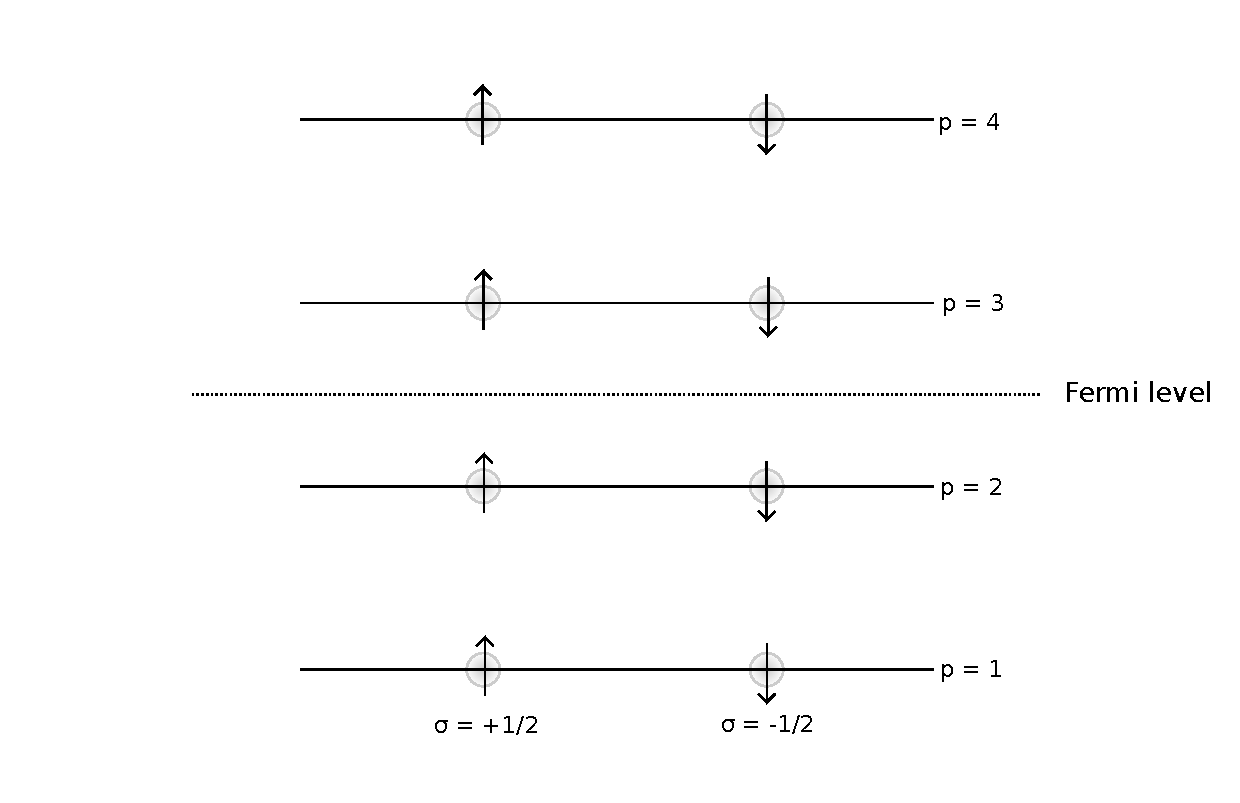
\includegraphics[width=\textwidth]{Figures/Pairing_model.pdf}
		\label{PairingModel_1}
		\caption{A figure depicting a 4 particles-4 holes state. The system consists of occupied particle states below the Fermi level and unoccupied hole states above Fermi level.}
	\end{figure}
	
	\begin{section}{The Hamiltonian}
		We limit ourselves to a two-body interaction, writing the Hamiltonian as
		\begin{align}
			\hat H = \sum_{\alpha \beta} \left< \alpha \right| \hat h_0 \left| \beta \right> \hat a_{\alpha}^{\dagger} \hat a_{\beta} 
			        + \frac{1}{4} \sum_{\alpha \beta \gamma \delta} \left< \alpha \beta \middle| \hat v_0 \middle| \gamma \delta \right> \hat a_{\alpha}^{\dagger} \hat a_{\beta}^{\dagger} \hat a_{\delta} \hat a_{\gamma}
		\end{align}
		We use the complete basis $\left| \alpha \right>$ and define the set as eigenvalues of the one-body operator, $\hat h_0$. 
		
		The system does require that the total spin is equal to $0$. In addition we will not allow spin pairs to be broken, i.e.\  singly excitated states are not allowed. 
		\begin{align}
			\left| \Psi_i^a \right> = 0 
		\end{align}	
		We introduce the double creation and annihilation operator. 
		\begin{align}
			\hat P_{pq}^{\dagger} = \hat a_{p \sigma}^{\dagger} \hat a_{p -\sigma}^{\dagger}
		\end{align}
		\begin{align}
			\hat P_{pq} =  a_{q \sigma} a_{q -\sigma}
		\end{align}

		We can rewrite the Hamiltonian as an unperterturbed part and a perturbation
		\begin{align}
			\hat H = \hat H_0 + \hat V
		\end{align}
		\begin{align}
			\hat H_0 = \xi \sum_{p \sigma} (p-1) \hat a_{p \sigma}^{\dagger} \hat a_{p \sigma}
		\end{align}
		\begin{align}
			\hat V = - \frac{1}{2}g \sum_{pq} \hat a_{p +}^{\dagger} \hat a_{p-}^{\dagger} \hat a_{q-} \hat a_{q+}
		\end{align}
		The value of $\xi$ determines the spacing between the energy levels, which I have set to $1$. This will not impact the insight attained solving this system. $p$ and $q$ determines the energy level. $\sigma$ is the spin, with value either $+\frac{1}{2}$ or $-\frac{1}{2}$. Both the unperturbed and perturbed Hamiltonian keeps total spin at $0$

		We can normal order the Hamiltonian by Wicks general theorem. 
		\begin{align}
			a_p^{\dagger} a_q = \left\{ a_p^{\dagger}a_q \right\} + \delta_{pq \in i}
		\end{align}
		\begin{align}
			a_p^{\dagger} a_q^{\dagger} a_s a_r = \left\{ a_p^{\dagger}a_q^{\dagger} a_s a_r \right\} +\left\{a_p^{\dagger}a_r\right\} \delta_{qs\in i} - \left\{a_p^{\dagger}a_s\right\} \delta_{qr\in i} \\
			+\left\{a_q^{\dagger}a_s\right\} \delta_{pr\in i} \
			- \left\{a_q^{\dagger}a_r\right\} \delta_{ps\in i} + \delta_{pr \in i} \delta_{qs \in i} - \delta_{ps \in i}\delta_{qr \in i}
		\end{align}
		Which gives the Normal-ordered Hamiltonian
		\begin{align}
			\hat H = \hat H_N + E_{ref}
		\end{align}
		\begin{align}
			\hat H_N = \hat F_N + \hat W 
		\end{align}
		\begin{align}
			\hat F_N =  \sum_{pq} h_{pq} \left\{ \hat a_{p \sigma}^{\dagger} \hat a_{p \sigma} \right\}
			- \sum_{pqi} \left< pi || qi \right> \left\{ \hat a_{p +}^{\dagger} \hat a_{q -} \right\}
		\end{align}
		\begin{align}
			\hat W = - \frac{1}{2} \sum_{pqrs} \left< pq || rs \right> \left\{ \hat a_{p +}^{\dagger} \hat a_{p-}^{\dagger} \hat a_{q-} \hat a_{q+} \right\}
		\end{align}
		\begin{align}
 			E_{ref} = \sum_{i} h_{ii} + \frac{1}{2} \sum_{ij} \left< ij \middle| \middle| ij \right>
		\end{align}

	\end{section}


	\begin{section}{Configuration Interaction theory}
		This system is a good way to benchmark various methods as we can compute the exact solution using Full Configuration Interaction. 

		\begin{figure}[h]
			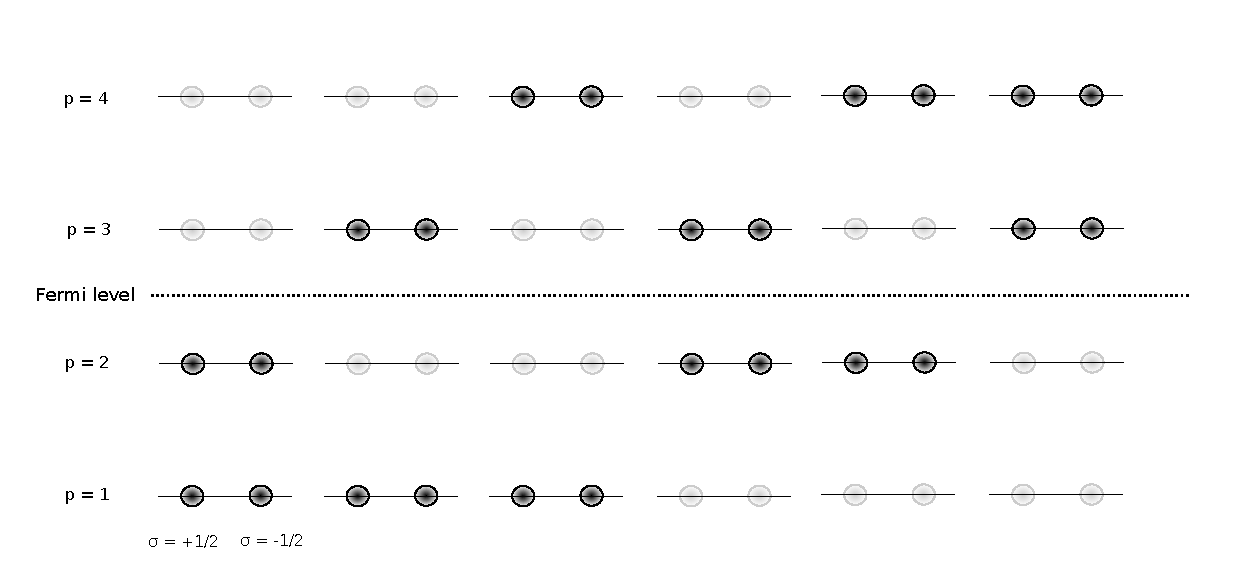
\includegraphics[width=1.1\linewidth]{Figures/Pairing_model2.pdf}
			\label{PairingModel_2}
			\caption{Configuration space for given pairing model showing all possible distributions of electrons}
		\end{figure}

	 	We need to diagonalize the Hamiltonian matrix looking at the linear combination of all different compinations of 
		\begin{align}
			\hat{ \mathcal{H} } = \left(  \begin{matrix}
				& \left| \Phi_0 \right> & \left| \Phi_{12}^{56} \right> & \left| \Phi_{12}^{78} \right> & \left| \Phi_{34}^{56} \right> & \left| \Phi_{34}^{78} \right> & \left| \Phi_{1234}^{5678} \right> \\ 
				\left< \Phi_0 \right| &   &   &   &   &   & \\
				\left< \Phi_{12}^{56} \right| &   &   &   &   &   & \\
				\left< \Phi_{12}^{78} \right| &   &   &   &   &   & \\
				\left< \Phi_{34}^{56} \right| &   &   &   &   &   & \\
				\left< \Phi_{34}^{78} \right| &   &   &   &   &   & \\
				\left< \Phi_{1234}^{5678} \right| &   &   &   &   &   & 
			\end{matrix} \right)
		\end{align}

		Excluding the 4p-4h excitations one does not diagonalize the exact matrix, but rather the approximated matrix known from Configuration Interaction. 

		The diagonal elements are calculated using Wick's theorem. Looking first at the ground state calculation with the unperturbed Hamiltonian part
		\begin{align}
			\left< \Phi_0 \middle| \hat{\mathbf{H_0}} \middle| \Phi_0 \right> 
		\end{align}
		\begin{align}
			\left< \right|  a_{2 \downarrow}  a_{2 \uparrow} a_{1 \downarrow} a_{1 \uparrow} \sum_{p \sigma} \delta (p-1) a_{p \sigma}^{\dagger} a_{p \sigma} 
			a_{1 \uparrow}^{\dagger} a_{1 \downarrow}^{\dagger} a_{2 \uparrow}^{\dagger} a_{2 \downarrow}^{\dagger} \left| \right> 
		\end{align}
		Which we see can contract in four different ways, resulting in 
		\begin{align}
			2 \delta (1-1) + 2 \delta (2-1) = 2 \delta
		\end{align}

		And the perturbation part
		\begin{align}
			\left< \Phi_0 \middle| \hat{\mathbf{V}} \middle| \Phi_0 \right>
		\end{align}
		\begin{align}
			\left< \right| a_{2 \downarrow}  a_{2 \uparrow} a_{1 \downarrow} a_{1 \uparrow} \left( -g / 2 \sum_{pq} a_{p \uparrow}^{\dagger} a_{q \downarrow}^{\dagger} a_{q \downarrow} a_{p \uparrow} \right) 
			a_{1 \uparrow}^{\dagger} a_{1 \downarrow}^{\dagger} a_{2 \uparrow}^{\dagger} a_{2 \downarrow}^{\dagger} \left| \right> 
		\end{align}
		As we can see, there are two ways this can contract, each contributing with the constant factor, $-g / 2$
		Resulting in the final Hamiltonian matrix 
		\begin{align}
			\hat{\mathcal{H}} = \left( \begin{matrix}
				2 \delta - g & -g / 2 & -g / 2 & -g / 2 & -g / 2 & 0  \\
				-g / 2 & 4 \delta - g & -g / 2 & -g / 2 & 0 & -g / 2  \\
				-g / 2 & -g / 2 & 6 \delta - g & 0 & -g / 2 & -g / 2 \\
				-g / 2 & -g / 2 & 0 & 6 \delta - g & -g / 2 & -g / 2 \\
				-g / 2 & 0 & -g / 2 & -g / 2 & 8 \delta - g & -g / 2 \\
				0 & -g / 2 & -g / 2 & -g / 2 & -g / 2 & 10 \delta - g 
			\end{matrix} \right)
		\end{align}

	\end{section}


	\begin{section}{Many-Body Perturbation Theory}
 		Given that our Hartree-Fock basis is canonical, $\hat F_N^0 = 0$, and $f_{pq} = \epsilon_p \delta_{pq}$, we can
 	\end{section}

 	\begin{section}{Canonical Hartree-Fock}
 		In the pairing model, we work with the Normal-ordered Hamiltonian
 		\begin{align}
 			\hat H_N = \hat F_N^d + \hat F_N^0 + \hat W		
 		\end{align}
 		Which is part of the total Hamiltonian by
 		\begin{align}
 			\hat H = \hat H_N + E_{\text{ref}}
 		\end{align}
 		Where
 		\begin{align}
 			\hat H_N \left| \Psi \right> = \Delta E \left| \Psi \right> 
 		\end{align}
 		If we use a Canonical Hartree-Fock basis, the Fock matrix will be diagonal, meaning 
 		\begin{align}
 			\hat F_N^o = 0 \;\;\; \text{     and  } \:\;\: f_{pq} = \epsilon_p \delta_{pq}
 		\end{align}
 		A noncanonical Hartree-Fock will be block diagonal with 
 		\begin{align}
 			f_{ia} = \left< i \right| \hat f \left| a \right> = 0
 		\end{align}

 	\end{section}

 	

 	

\end{chapter}




\begin{chapter}{Infinite Matter}
	A study of infinite matter is the most comprehensible way of studying nuclear material. This thesis will study the infinite electron gas before the final study of nuclear material. This is done because of pedagogical reasons and because the electron gas has closed form solutions that provide important benchmarking for the code. 
	\begin{section}{The Infinate Electron Gas}
		The infinite electron gas gives a good approximation to valence electrons in metal. The gas consist only of interacting electrons with a uniform background of charged ions. The whole system is charge neutral. We assume a finite cubic box as done in \cite{Shepherd2012} and \cite{Shepherd2013}. The box has a length $L$ and volume $\Omega = L^3$, with $N_e$ as the number of electrons with a charge density $\rho = N_e / \Omega$.

		\begin{subsection}{The Hamiltonian}
			The electrons interact with the sentral symmetric Colomb potential, $\hat V(\vec r_1, \vec r_2)$ depending only on the distance $\left| \vec r_1 - \vec r_2 \right|$. The Hamiltonian for infinite electron gas is \cite{Baardsen}
			\begin{align}
				\hat H = \hat H_1 + \hat H_2 = \hat H_{\text{kin}} + \hat H_{\text{interaction}}
			\end{align}
			The interaction term will be dependent on both the electron-electron interaction, the electron-background interaction and the background-background interaction
			\begin{align}
				\hat H = \hat H_{\text{kin}} + \hat H_{\text{ee}} + \hat H_{\text{eb}} + \hat H_{\text{bb}}
			\end{align}
			And the kinetic energy, $\hat H_{\text{kin}}$ is given as
			\begin{align}
				\hat H_{\text{kin}} = \sum_p \frac{\hbar ^2 k^2}{2m} a_{k \sigma}^{\dagger} a_{k \sigma}
			\end{align}
			The background-interaction terms will vanish as explained by Fraser et al \cite{Fraser et al} both for three- and two-dimensional electron gas. When we sum over all particles, we can write the electron-electron interaction term as an Ewald summation term, because it is not possible to use a $1/r$ term for infinite systems \cite{Drummond2008} \cite{MHJonline}. We can write this term as
			\begin{align}
				\hat H_{ee} = \sum_{i<j}^N v_E(\mathbf{r}_i - \mathbf{r}_j) + \frac{1}{2}Ne^2v_0
			\end{align}
			Where $v_E(\mathbf{r})$ is an effective two-body interaction. $v_0$ is the self-interaction term, defined as 
			\begin{align}
				v_0 = \lim_{\mathbf{r}\rightarrow \infty} \left\{ v_E(\mathbf{r}) - \frac{1}{r} \right\}
			\end{align}
			The Ewald summation will account for interactions between all electrons in the finite size system as well as all the image electrons that will arize from self-interaction because of periodic boundaries. We define it as 
			\begin{align}
				v_E(\mathbf{r}) &= \sum_{k \neq 0} \frac{4\pi}{L^3k^2} e^{i \mathbf{k}\cdot \mathbf{r} } e^{-\eta^2 k^2 / 4} \\
								&+ \sum_{\mathbf{R}} \frac{1}{|	\mathbf{r} - \mathbf{R}|} \text{erfc} \left( \frac{| \mathbf{r} - \mathbf{R}|}{\eta} \right) - \frac{\pi \eta^2}{L^3}
			\end{align}
			$L$ is the size of the box, $\mathbf{k}$ is the momentum vector, while $\mathbf{r}$ represent the position vectors for all electrons. The translational vector $\mathbf{R}$ is used to obtain all image cells in the entire real space \cite{MHJonline}
			\begin{align}
				\mathbf{R} = L(n_x \mathbf{u}_x + n_y \mathbf{u}_y + n_z \mathbf{u}_z)
			\end{align}
			We have used the error functions
			\begin{align}
				\text{erf}(x) = \frac{2}{\sqrt{\pi}} \int_0^x e^{-t^2} \text{dt}
			\end{align}
			\begin{align}
				\text{erfc}(x) = 1 - \text{erf}(x) = \frac{2}{\sqrt{\pi}} \int_x^\infty e^{-t^2} \text{dt}
			\end{align}
			We use this relation because an interaction on the form $1/|r|$ is not convergent for an infinite number of particle \cite{Audun}. Ewald found that one can rewrite the interaction in terms of these error functions \cite{Ewald}
			\begin{align}
				\frac{1}{r} = \frac{\text{erf}(\frac{1}{2}\sqrt{\eta}r)}{r} + \frac{\text{erfc}(\frac{1}{2}\sqrt{\eta}r)}{r}
			\end{align}
			One can calculate the two-dimensional Ewald term as well \cite{Baardsen}, resulting in 
			\begin{align}
				v_E^{\eta=0, z=0} = \sum_{\mathbf{k} \neq 0} \frac{2 \pi}{L^2 k} e^{i \mathbf{k} \cdot \mathbf{r}_{xy}}
			\end{align}
		\end{subsection}
		
		\begin{subsection}{The Reference Energy}
			The reference energy for electron gas can be written as \cite{Baardsen}
			\begin{align}
				E_{\text{ref}} = \sum_i \left<i | h_0 | i\right> + \frac{1}{2} \sum_{ij} \left<ij||ij\right> + \frac{1}{2} Av_0
			\end{align}
			$A$ is the number of electrons, and the term $A v_0$ is the so-called Madelung constant. It is how we incorporates the self-interaction term into the system. This factor will be larger for smaller system and vanish as we approach the thermodynamic limit. 
		\end{subsection}
		
		\begin{subsection}{The Fock Matrix Elements}
			The Fock Matrix Elements will be given as
			\begin{align}
				\left< p | f | q \right> = \frac{k_p^2}{2m} \delta_{\mathbf{k}_p \mathbf{k}_q} \delta_{m_{s_p} m_{s_q}} + \sum_i \left<pi||qi\right>
			\end{align}
			We notice that the Fock Matrix elements can be written as a diagonal part plus the $\hat U$ operator. As we can see from (\ref{3.93}) and (\ref{3.95}), this means the perturbation can be written solely by the two-body interaction
			\begin{align}
				\hat V = \frac{1}{4} \sum_{pqrs} \left<pq||rs\right> \hat p^\dagger \hat q^\dagger \hat s \hat r
			\end{align}
		\end{subsection}

		\begin{subsection}{Anti-Symmetric Matrix Elements}
			We now need to define the matrix elements for the two- and three-dimensional electron gas to calculate the perturbation 
			\begin{align}
				&\left< \mathbf{k}_p m_{s_p} \mathbf{k}_q m_{s_q} || \mathbf{k}_r m_{s_r} \mathbf{k}_s m_{s_s} \right> \\
				&= \frac{4 \pi e^2}{L^3} \delta_{\mathbf{k}_p + \mathbf{k}_q, \mathbf{k}_r + \mathbf{k}_s} \left\{ \delta_{ m_{s_p},m_{s_r} } \delta_{ m_{s_q},m_{s_s} } (1 - \delta_{\mathbf{k}_p, \mathbf{k}_r}) \frac{1}{| \mathbf{k}_r - \mathbf{k}_p|^2} \right. \\
				& - \delta_{ m_{s_p},m_{s_s} } \delta_{ m_{s_q},m_{s_r} } (1 - \delta_{\mathbf{k}_p, \mathbf{k}_s}) \left. \frac{1}{| \mathbf{k}_s - \mathbf{k}_p|^2}  \right\}
			\end{align}
			The two-dimensial case is almost identical
			\begin{align}
				&\left< \mathbf{k}_p m_{s_p} \mathbf{k}_q m_{s_q} || \mathbf{k}_r m_{s_r} \mathbf{k}_s m_{s_s} \right> \\
				&= \frac{2 \pi e^2}{L^2} \delta_{\mathbf{k}_p + \mathbf{k}_q, \mathbf{k}_r + \mathbf{k}_s} \left\{ \delta_{ m_{s_p},m_{s_r} } \delta_{ m_{s_q},m_{s_s} } (1 - \delta_{\mathbf{k}_p, \mathbf{k}_r}) \frac{1}{| \mathbf{k}_r - \mathbf{k}_p|} \right. \\
				& - \delta_{ m_{s_p},m_{s_s} } \delta_{ m_{s_q},m_{s_r} } (1 - \delta_{\mathbf{k}_p, \mathbf{k}_s}) \left. \frac{1}{| \mathbf{k}_s - \mathbf{k}_p|}  \right\}
			\end{align}		
		\end{subsection}

		\begin{subsection}{The Plane Wave Basis}
			When set up with periodic boundary conditions, the Homogenous electron gas can be set up with free particle normalized wave functions
			\begin{align}
				\psi_{\vec k \sigma} (\vec r) = \frac{1}{\sqrt{\Omega}} e^{i \vec k \vec r} \xi_{\sigma}
			\end{align}
			Where $\vec k$ is the wave number and $\xi_{\sigma}$ is a spin function. 
			\begin{align}
				\xi_{+\frac{1}{2}} = \left( \begin{matrix} 1 \\ 0 \end{matrix} \right) \:\;\:\; \xi_{-\frac{1}{2}} = \left( \begin{matrix} 0 \\ 1 \end{matrix} \right)
			\end{align}
			Because of periodic boundary conditions, we acquire the following wave numbers
			\begin{align}
				k_i = \frac{2\pi n_i}{L} \:\:\:\;\; i = x,y,z \;\;\:\:\: n_i = 0, \pm 1, \pm 2, ...
			\end{align}
			and the associated single-particle energies for two dimensions
			\begin{align}
				\epsilon_{n_x,n_y} = \frac{\hbar^2}{2m} \left( \frac{2\pi}{L} \right)^2 (n_x^2 + n_y^2)
			\end{align}
			And for three dimensions
			\begin{align}
				\epsilon_{n_x,n_y,n_z} = \frac{\hbar^2}{2m} \left( \frac{2\pi}{L} \right)^2 (n_x^2 + n_y^2 + n_z^2 )
			\end{align}
			By the nature of the single particle energies, the energy levels will be determined by the value of $n_x^2 + n_y^2 + n_z^2$. There are different combinations of $n_x, n_y$ and $n_z$ that set up each energy level. The cumulative number of particles needed to completely fill these energy states will be named \textit{magic numbers} and are listed in table (\ref{Magic Numbers 3d}). 
			\begin{table}[H]
				\begin{center}
					\begin{tabular}[center]{l | c c c | c | c | r }
						$n_x^2 + n_y^2 + n_z^2$ & $n_x$ & $n_y$ & $n_z$ & $N_{\uparrow \uparrow}$ & $N_{\uparrow \downarrow}$ & $N_{\uparrow \downarrow} \hat \tau$ \\
						\hline
						0 & 0 & 0 & 0 & 1 & 2 & 4 \\
						\hline
						1 & 1 & 0 & 0 &   &   &   \\
						  & -1& 0 & 0 &   &   &   \\
						  & 0 & 1 & 0 &   &   &   \\
						  & 0 & -1& 0 &   &   &   \\
						  & 0 & 0 & 1 &   &   &   \\
						  & 0 & 0 & -1& 7 & 14& 28\\
						\hline
						2 & 1 & 1 & 0 &   &   &   \\
						  & 1 & -1& 0 &   &   &   \\
						  & 1 & 0 & 1 &   &   &   \\
						  & 1 & 0 & -1&   &   &   \\
						  & -1& 1 & 0 &   &   &   \\
						  & -1& -1& 0 &   &   &   \\
						  & -1& 0 & 1 &   &   &   \\
						  & -1& 0 & -1&   &   &   \\
						  & 0 & 1 & 1 &   &   &   \\
						  & 0 & 1 & -1&   &   &   \\
						  & 0 & -1& 1 &   &   &   \\
						  & 0 & -1& -1&19 &38 & 76\\
						\hline
						3 & 1 & 1 & 1 &   &   &   \\
						  & 1 & 1 & -1&   &   &   \\
						  & 1 & -1& 1 &   &   &   \\
						  & 1 & -1& -1&   &   &   \\
						  & -1& 1 & 1 &   &   &   \\
						  & -1& 1 & -1&   &   &   \\
						  & -1& -1& 1 &   &   &   \\
						  & -1& -1& -1&27 & 54&108\\
						\hline
						4 & 2 & 0 & 0 &   &   &   \\
						  & -2& 0 & 0 &   &   &   \\
						  & 0 & 2 & 0 &   &   &   \\
						  & 0 & -2& 0 &   &   &   \\
						  & 0 & 0 & 2 &   &   &   \\
						  & 0 & 0 & -2& 33& 66&132\\
						\hline
						5 &   &   &   & 57&114&228\\
						\hline
						6 &   &   &   & 81&162&324\\
						\hline
						7 &   &   &   & 81&162&324\\
						\hline
						8 &   &   &   & 93&186&372
					\end{tabular}
				\end{center}
				\caption{All magic numbers for three dimensional infinite matter. The table demonstrates how states will fill up energy levels. $n_x$, $n_y$ and $n_z$ represent momentum quantum numbers, $n_x^2 + n_y^2 + n_z^2$ represent energy level. $N_{\uparrow \uparrow}$ shows magic number without spin degeneracy, $N_{\uparrow \downarrow}$ adds two possible spins, and $N_{\uparrow \downarrow} \hat \tau $ also adds isospin degeneracy.} 
				\label{Magic Numbers 3d}
			\end{table}

		\end{subsection}

	\end{section}

	\begin{section}{Infinite Nuclear Matter}
		Central to my thesis, is the study of infinite nuclear matter. I look at baryonic matter similar to the dense baryonic matter found in neutron stars. I limit the study to temperatures far below Fermi level. The matter is mostly made up of an equilibrium of baryons and leptons. In neutron star matter, we assume the equilibrium consist of protons, neutrons, electrons and muons with densities larger than $0.1 \text{fm}^-3$. The equilibrium conditions are specified by weak interactions
		\begin{align}
		 	b_1 \rightarrow b_2 + l + \bar \nu_l \:\:\:\:\:\: b_2 + l \rightarrow b_1 + \nu_l
		\end{align} 
		Where $b$ represent either neutron or proton and $l$ is either an electron or muon. $\nu_l$ is the corresponding neutrino. 

		Nuclear matter is a hypothetical system filling all of space at a uniform density. Symmetric nuclear matter (SNM) consist of equal numbers of protons of neutrons, while pure nuclear matter (PNM) consist only of neutrons. For finite-nucleus systems, the most difficult part is calculating the single particle wave function. For nuclear matter we can use plane wave basis and similar to electron gas, the difficult part is calculating the energy and the effective interaction between particles \cite{Day1967}. In my calculations, I have looked at pure nuclear matter. 


	\end{section}
	\begin{section}{Nuclear Interaction}
		Nuclear matter is composed of baryons, which interacts through the strong force. 
		
		\begin{subsection}{The Minnesota Potential}
			The Minnesota Potential is given as
			\begin{align}
				v(r) = &\left(v_R + (1 + P_{12}^\sigma) v_T/2 + (1 - P_{12}^\sigma) v_S/2 \right) \\
					   \cdot &\left( \alpha + (2- \alpha)P_{12}^r \right)/2 + (1+m_{t,1})(1+m_{t,2})\frac{e^2}{4r}
			\end{align}
			where $r$ is given as $\left| \mathbf{r_1} - \mathbf{r_2} \right|$ and $m_t$ is the isospin projection of particle 1 or 2. $m_t = \pm 1$. 
			$P_{12}^\sigma $ and $P_{12}^r$ are exchange operators for spin and position, respectively \cite{Baardsen}. Furthermore, we have used
			\begin{align} 
				v_R = v_{0R}e^{-k_R r^2}, \:\:\: v_T = -v_{0T} e^{-k_Tr^2}, \:\:\: v_S = -v_{0S}e^{-k_sr^2}
			\end{align}
			Where the constants $v_{0R}$, $v_{0T}$, $v_{0S}$, $k_R$, $k_T$ and $k_S$ are given by \cite{Thompson1977}
			\begin{enumerate}
				\item $v_{0R} = 200$MeV,  $k_R = 0.1487 \text{fm}^{-2}$
				\item $v_{0T} = 178$MeV,  $k_T = 0.649 \text{fm}^{-2}$
				\item $v_{0S} = 91.85$MeV, $k_S = 0.465 \text{fm}^{-2}$
			\end{enumerate}
			Written by second quantisation, we want to calculate the two-body interaction
			\begin{align}
			 	\left<k_p k_q \middle| v \middle| k_r k_s \right> = \frac{V_0}{L^3} \left(\frac{\pi}{\alpha}\right)^{3/2} e^{-q^2 / 4 \alpha} \delta_{\vec k_p + \vec k_q, \vec k_r + \vec k_s}
			\end{align}
			Where $q$ is the relative momentum transfer
			\begin{align}
				\mathbf{q} = \mathbf{p} - \mathbf{p'} 
			\end{align}
			\begin{align}
				\mathbf{p} = \frac{1}{2} (\mathbf{k}_p - \mathbf{k}_q) \:\:\:\:\: \mathbf{p'} = \frac{1}{2}(\mathbf{k}_r- \mathbf{k}_s) 
			\end{align}
			We can now set up the two-body Matrix-elements for the Minnesota Potential
			\begin{align}
				\left<\mathbf{k}_p \mathbf{k}_q \middle| v \middle| \mathbf{k}_r \mathbf{k}_s \right> = 
				&\left<\mathbf{k}_p \mathbf{k}_q \right| \frac{1}{2} \left( V_R + \frac{1}{2} V_T + \frac{1}{2} V_S \right) \left| \mathbf{k}_r \mathbf{k}_s \right>  \\
				+&\left<\mathbf{k}_p \mathbf{k}_q \right| \frac{1}{4} (V_T - V_S) P_{12}^\sigma \left| \mathbf{k}_r \mathbf{k}_s \right> \\
				-&\left<\mathbf{k}_p \mathbf{k}_q \right| \frac{1}{2} \left( V_R + \frac{1}{2} V_T + \frac{1}{2} V_S \right) P_{12}^\sigma P_{12}^\tau \left| \mathbf{k}_r \mathbf{k}_s \right> \\
				-&\left<\mathbf{k}_p \mathbf{k}_q \right| \frac{1}{4}(V_T - V_S) P_{12}^\tau  \left| \mathbf{k}_r \mathbf{k}_s \right>&
			\end{align}
			Matrix elements for the spin and isospin exchange operators are 
			\begin{align}
				\left< \sigma_p \sigma_q \right| P_{12}^\sigma \left| \sigma_r \sigma_s \right> = \delta_{\sigma_p,\sigma_s} \delta_{\sigma_q,\sigma_r}
			\end{align}
			One can see that these matrix elements come at a far greater computational cost than for electron-electron interaction in the electron gas. Therefore it is necessary to compute and store all elements instead of computing them "on the fly". Source: Lecture 1-2 infinite matter. 
		\end{subsection}
		
	\end{section}
\end{chapter}




\begin{chapter}{Implementation}
	In this thesis I have created three different solvers for Coupled Cluster Doubles equations. 
	\begin{enumerate}
		\item A naive brute force implementation of the equations summing over all variables. 
		\item A naive brute force implementation of intermediate equations summing over all variables.
		\item Rewriting summations as matrix-matrix multiplications and exploiting various symmetry arguments one can set up a block implementation.
	\end{enumerate}	
	There is a significant performance leap between each method, but I have included the first two solvers for both educational and benchmarking purposes. The Pairing model with 4 particles and 4 holes is a small system that one can easily solve using the naive approach. After producing expected results with the naive solver, I have compared the more complicated solvers to the naive solver for all systems. 

	\begin{section}{Implementing the CCD equations}
		The basic steps of all implemented CCD algorithms can be explained through these steps
		\begin{enumerate}
			\item Initialize amplitudes $t^{(0)} = 0$ and $\Delta E_{CCD}^{(0)} = 0$
			\item Update the amplitudes and calculate $\Delta E_{CCD}^{(1)}$
			\item If $ |\Delta E_{CCD}^{(1)} - \Delta E_{CCD}^{(0)}| \geq \epsilon $, update amplitudes and compute $\Delta E_{CCD}^{2}$
			\item Repeat until $ |\Delta E_{CCD}^{(n+1)} - \Delta E_{CCD}^{(n)}| \leq \epsilon $
		\end{enumerate}
		The difference between the three solvers I have implemented is the way I update amplitudes. The naive brute force solver loops over all indices when computing. An example of diagram $L_a$ is shown below

		\begin{lstlisting}
		for i in 0, ..., Nholes:
			for j in 0, ..., Nholes:
				for a in Nholes, ..., Nparticles:
					for b in Nholes, ..., Nparticles:
						for c in Nholes, ..., Nparticles:
							for d in Nholes, ..., Nparticles:
								tnew(a,b,i,j) = 0.5  v(a,b,c,d)  told(c,d,i,j)
		\end{lstlisting}

		A significant cost reduction can be obtained by factorizing the diagrams as shown in equation (\ref{Intermediates}). By calculating the four intermediate diagrams, $I_1$, $I_2$, $I_3$ and $I_4$ beforehand and storing the results reduce the cost of calculation from $\mathcal{O}(h^4 p^4)$ to $\mathcal{O}(h^4 p^2)$. The second solver applies this method. 

	\end{section}

	\begin{section}{Matrix Representation of Contractions}
		Diagrams can be viewed as contractions of tensors of varying degree. An example is the matrix-matrix multiplication product
		\begin{align}
		 	\left( M N \right)_{\gamma}^{\alpha} = \sum_{\beta} M_{\beta}^\alpha N_\gamma^\beta 
		 	\label{matrix matrix multiplication}
		\end{align} 

		As our goal is to rewrite the Coupled Cluster equations as matrix-matrix products. We will need to map tensors of rank $\geq 2$ onto matrices. One mapping that provides systematic and unique matrix elements can be 
		\begin{align}
			\left<pq\middle| \hat v\middle|rs\right> = V_{\alpha(p,q),\beta(r,s)}
		\end{align}
		Where 
		\begin{align}
			\alpha(p,q) = p + q N_p \;\,\:\; \beta(r,s) = r + s N_r
			\label{mapping of matrix elements}
		\end{align}
		We need to be careful when mapping tensors this way. Consider first the calculation of the perfectly aligned $L_a$ term
		\begin{align}
			L_a = \sum_{cd} \left< ab \middle| \hat v\middle|cd\right> t_{ij}^{cd}
		\end{align}
		Mapping this equation using equation (\ref{mapping of matrix elements})
		\begin{align}
			\left< ab \middle| \hat v\middle|cd\right> = v_{ab}^{cd} \rightarrow V_{\beta(c,d)}^{\alpha(a,b)}
		\end{align}
		and
		\begin{align}
			t_{ij}^{cd} \rightarrow T_{\delta(i,j)}^{\beta(c,d)}
		\end{align}
		As we are mapping to unique elements 
		\begin{align}
			\beta(c,d) = \beta(c,d)
		\end{align}
		We can now rewrite the equation 
		\begin{align}
			(L_a)_ \delta^\alpha = \sum_ \beta V_ \beta^\alpha T_ \delta^\beta
		\end{align}
		Implying by regarding equation (\ref{matrix matrix multiplication}) that we can rewrite the product as matrix-matrix multiplication 
		\begin{align}
			L_a = VT
		\end{align}

		\begin{subsection}{Aligning elements}	
			Unfortunately, not all product are perfectly aligned like $L_a$. Consider, for example, the term, $L_c$
			\begin{align}
				L_c = -P\left(ij\middle|ab\right) \sum_{kc} \left<kb\middle|\hat v\middle|cj\right>t_{ik}^{ac}
			\end{align}
			Using the same mapping scheme
			\begin{align}
				\left<kb\middle|\hat v\middle|cj\right> = v_{cj}^{kb} \rightarrow V_{\beta(cj)}^{\alpha(kb)}
			\end{align}
			and
			\begin{align}
				t_{ik}^{ac} \rightarrow T_{\delta(ik)}^{\gamma(ac)}
			\end{align}
			This matrix multiplication is misaligned, and if the number of particles is unequal to the number of holes, the matrices' size will uncompatible. 
			\begin{align}
				(L_c)_ \delta^\alpha \neq -P\left(ij\middle|ab\right) \sum_ \beta V_{\beta(cj)}^{\alpha(kb)} T_{\delta(ik)}^{\gamma(ac)}
			\end{align}
			We need to find another mapping, such that
			\begin{align}
				v_{cj}^{kb} \rightarrow \tilde V_{\beta(ck)}^{\alpha(bj)}
			\end{align}
			and 
			\begin{align}
				t_{ik}^{ac} \rightarrow \tilde T_{\delta(ia)}^{\gamma(ck)}
			\end{align}
			Now, the matrix multiplication is aligned
			\begin{align}
				(\tilde L_c)_ \delta^\alpha = -P\left(ij\middle|ab\right) \sum_ \beta \tilde V_{\beta(ck)}^{\alpha(bj)} \tilde T_{\delta(ia)}^{\gamma(ck)}
			\end{align}
			Note, however, that 
			\begin{align}
				L_c \neq \tilde L_c
			\end{align}
			We must "realign" $\tilde L_c$ to match the correct diagram
			\begin{align}
				(\tilde L_c)_{\delta(i,a)}^{\alpha(b,j)} \rightarrow (L_c)_{\delta(i,k)}^{\alpha(k,b)}
			\end{align}

			Another example is the $Qc$ term
			\begin{align}
				Q_c = -\frac{1}{2} \hat P(ij) \sum_{klcd} \left< kl \middle| v \middle| cd \right> t_{ik}^{ab} t_{jl}^{cd} 
			\end{align}
			We can rewrite this as a matrix-matrix multiplication with the matrix elements given by
			\begin{align}
				\left< kl \middle| v \middle| cd \right> = v_{cd}^{kl} & \rightarrow V^{\alpha(cd)}_{\beta(kl)} \\
				t_{ik}^{ab} & \rightarrow (T_1)_{\gamma(ik)}^{\delta(ab)} \\
				t_{jl}^{cd} & \rightarrow (T_2)_{\omega(jl)}^{\eta(cd)}
			\end{align}
			Because we sum over the coefficients $klcd$, we must make sure that they belong to the "inner" indexes. This can only be done by creating a hole, particle-particle-hole configuration. We must also change the order of multiplication
			\begin{align}
				V^{\alpha(cd)}_{\beta(kl)} &  \rightarrow \tilde V^{\delta(k)}_{\gamma(cdl)} \\
				(T_1)_{\gamma(ik)}^{\delta(ab)} & \rightarrow \tilde (T_1)^{\alpha(abi)}_{\delta(k)} \\
				(T_2)_{\omega(jl)}^{\eta(cd)} & \rightarrow \tilde (T_2)^{\gamma(cdl)}_{\beta(j)}
			\end{align}
			This gives us
			\begin{align}
				( \tilde Q_c )_{\beta(j)}^{\alpha(abi)} = -\frac{1}{2} \hat P(ij) \sum_{klcd} (\tilde T_1)^{\alpha(abi)}_{\delta(k)} \tilde V^{\delta(k)}_{\gamma(cdl)} (\tilde T_2)^{\gamma(cdl)}_{\beta(j)}
			\end{align}
			Which must be realigned back to the properly aligned $Q_c$ before it can be added to the amplitude equations.
			\begin{align}
				( \tilde Q_c )_{\beta(j)}^{\alpha(abi)} \rightarrow (Q_c)_{\beta(ij)}^{\alpha(ab)}
			\end{align}
			We will need a general mapping function that can be used regardless of the amount of states used. It turns out that we can use the same mapping as before, just generalized to $N$ states.
			\begin{align}
				\alpha(p_1,p_2,p_3,...,p_N) = p_1 + p_2N_1 + p_3N_1N_2 + ... + p_N N_1 N_2 ... N_{N-1} 
			\end{align}
			Where $N_n$ determines the maximum number of states for $p_n$. If for example $p_n \in i$, i.e. $p_n$ is a hole-state, $N_n = N_{holes}$.

			Writing the diagrams as matrix-matrix multiplications serves as a significant reduction of computational time, due to the efficient algortithms in the BLAS-packages for matrix-matrix multiplications. However, since one has to save all the matrices, memory usage will be a problem for large basises. 
		\end{subsection}

	\end{section}

	\begin{section}{Block Implementation}
		One can both greatly reducing memory usage and improve computational speed by exploiting symmetries for infinite matter . Due to kroenecker delta's in the interaction, one such symmetry is the conservation of momentum
		\begin{align}
			\delta_{\vec k_p + \vec k_q, \vec k_r + \vec k_s} \rightarrow \vec k_p + \vec k_q = \vec k_r + \vec k_s
		\end{align}
		We also conserve spin 
		\begin{align}
			m_{s_p} + m_{s_q} = m_{s_r} + m_{s_s}
		\end{align}
		and for nuclear matter, we will conserve isospin aswell
		\begin{align}
			m_{t_p} + m_{t_q} = m_{t_r} + m_{t_s}
		\end{align}
		The amplitudes will be subject to the same restrictions, vizualised by the first order amplitude generated by perturbation theory
		\begin{align}
			(t_{ij}^{ab})^{t=0} = \frac{\left<ab\middle|\hat v\middle|ij\right>}{\epsilon_i + \epsilon_j - \epsilon_a - \epsilon_b}
		\end{align}
		Looking at the $L_a$ term
		\begin{align}
			L_a = \sum_{cd} \left<ab\middle|\hat v\middle|cd\right> t_{ij}^{ab}
		\end{align}
		We see that 
		\begin{align}
			\vec k_a + \vec k_b = \vec k_c + \vec k_d = \vec k_i + \vec k_j
		\end{align}
		And the same for spin
		\begin{align}
			m_{s_a} + m_{s_b} = m_{s_c} + m_{s_d} = m_{s_i} + m_{s_j} 
		\end{align}
		When summing over all variations of contractions, only the quantum numbers preserving the symmetry requirements are nonzero. When storing the interactions in a matrix, most of it will have zero-elements. The blocking method will store the nonzero parts in blocks inside the matrix. By keeping track of the blocks, we can reduce the full matrix-matrix multiplication to a series of multiplications of the blocks. We will hereby refer to the series of blocks as \textit{channels}.

		\begin{subsection}{Two-state configurations}
			As we can see from the $L_a$ diagram, the conservation laws apply for a combination of two states. The next step is then to set up all two-state configurations that will be needed. We start by setting up the direct two-state channels, $T$, which consist of all two-hole and two-particle configurations. A unique identifier must be set up for the combination of quantum numbers. The identifier is used to aligning the non-zero combinations of two-body states to the same channel. Without this identifier, we will have to loop over all channels for each two-body state. I have used the following function 
			\begin{align}
				\text{Index}(N_x,N_y,N_z,S_z,T_z) = &2(N_x + m)M^3 + 2(N_y+m)M^2 + \\ & 2(N_z+m)M + 2(S_z+1) + (T_z+1)
			\end{align}
			Using the same logic as in equation (\ref{mapping of matrix elements}) to get a unique identifier for every combination of $N_x,N_y,N_z,S_z$ and $T_z$. Which imply that the two-body states have the same momentum, spin and isospin projection, which satisfies our conservation laws. We need $m$ and $M$ to be sufficiently large. I have used
			\begin{align}
				m = 2|\sqrt{N_{\text{max}}}| \:\:\:\:\:\: M = 2m +1
			\end{align}
			Because of the Pauli-exclusion, two particles cannot occupy the same state, so we can further reduce the amount of two-body states by excluding equal one-body states from the channels. An algorithm for setting up the direct channels can be portraied as
			\begin{align*}
				&\mathbf{for } \text{ one-body state 1} \in \text{STATES}: \\
				&\:\:\:\: \mathbf{for } \text{ one-body state 2} \in \text{STATES}: \\
				&\:\:\:\:\:\:\:\: \mathbf{if} \text{ one-body state 1} \neq \text{ one-body state 2}: \\
				&\:\:\:\:\:\:\:\:\:\: N_x = n_{x,1} + n_{x,2} \\
				&\:\:\:\:\:\:\:\:\:\: N_y = n_{y,1} + n_{y,2} \\
				&\:\:\:\:\:\:\:\:\:\: N_z = n_{z,1} + n_{z,2} \\
 				&\:\:\:\:\:\:\:\:\:\: S_z = m_{s,1} + m_{s,2} \\
				&\:\:\:\:\:\:\:\:\:\: T_z = m_{t,1} + m_{t,2} \\
				&\:\:\:\:\:\:\:\:\:\: \text{Id} = \text{Index}(N_x,N_y,N_z,S_z,T_z) \\
				&\:\:\:\:\:\:\:\:\:\: T \leftarrow (\text{ one-body state 1}, \text{ one-body state 2}, \text{ Id})
			\end{align*}

		\end{subsection}
		
		\begin{subsection}{Unaligned channels}
			Diagram $L_a$, $L_b$ and $Q_a$ have conservation requirements as shown previously for $L_a$
			\begin{align}
			 	\mathbf{k}_a + \mathbf{k}_b = \mathbf{k}_c + \mathbf{k}_d = \mathbf{k}_i + \mathbf{k}_j 
			\end{align}
			Which are implemented using the direct channels. We will however run into some trouble when computing the unaligned diagrams $L_c$, $Q_b$, $Q_c$ and $Q_d$. The $L_c$ diagram is given by 
			\begin{align}
				L_c = - \hat P(ij|ab) \sum_{kc} \left<kb\middle|\hat v\middle| cj \right> t_{ik}^{ac}
			\end{align}
			Looking at the conservation requirement for $L_c$
			\begin{align}
				\mathbf{k}_k + \mathbf{k}_b = \mathbf{k}_c + \mathbf{k}_j = \mathbf{k}_a + \mathbf{k}_c = \mathbf{k}_i + \mathbf{k}_k
			\end{align}
			and 
			\begin{align}
				m_{s,k} + m_{s,b} = m_{s,c} + m_{s,j}  \:\:\:\:\:\:\: m_{t,k} + m_{t,b} = m_{t,c} + m_{t,j} 
			\end{align}
			When realigning the equation, we want it to be
			\begin{align}
				\tilde Lc = -\hat P(ij|ab) \sum_{kc} \left<bj | \tilde v | ck \right> \left< ck \right| \tilde t \left| ai \right>
			\end{align}
			We reorganize the conservation requirements as well to make sure we only calculate the non-zero terms
			\begin{align}
				\mathbf{k}_b - \mathbf{k}_j = \mathbf{k}_c - \mathbf{k}_k = \mathbf{k}_c - \mathbf{k}_k = \mathbf{k}_i - \mathbf{k}_a
			\end{align}
			Spin and isospin will be subject to the same reorganizing. We see that the direct channels do not represent the right conservation requirement and we must set up the cross channels, $X$, that consist of particle-hole or hole-particle two-body configurations. An algorithm can be set up as
			\begin{align*}
				&\mathbf{for } \text{ one-body state 1} \in \text{STATES}:\\
				&\:\: \mathbf{for } \text{ one-body state 2} \in \text{STATES}:\\
				&\:\:\:\: \mathbf{if} \text{ one-body state 1} \neq \text{ one-body state 2}:\\
				&\:\:\:\:\:\: N_x = n_{x,1} - n_{x,2} \\
				&\:\:\:\:\:\: N_y = n_{y,1} - n_{y,2} \\
				&\:\:\:\:\:\: N_z = n_{z,1} - n_{z,2} \\
 				&\:\:\:\:\:\: S_z = m_{s,1} - m_{s,2} \\
				&\:\:\:\:\:\: T_z = m_{t,1} - m_{t,2} \\
				&\:\:\:\:\:\: \text{Id} = \text{Index}(N_x,N_y,N_z,S_z,T_z) \\
				&\:\:\:\:\:\: X \leftarrow (\text{ one-body state 1}, \text{ one-body state 2}, \text{ Id}) \\
				&\:\:\:\:\:\: \text{Id}' = \text{Index}(-N_x,-N_y,-N_z,-S_z,-T_z) \\
				&\:\:\:\:\:\: X' \leftarrow (\text{ one-body state 2}, \text{ one-body state 1}, \text{ Id'})
			\end{align*}
			Where $X'$ is the cross channel compliment, $X(pq) = X'(qp)$. The coss-channels are used for calculating $Q_b$ and $L_c$. 

			Looking at the diagram $Q_c$
			\begin{align}
				Q_c = -\frac{1}{2} \hat P(ij) \sum_{klcd} \left<kl|\hat v|cd\right> t_{ik}^{ab} t_{jl}^{cd}
			\end{align}
			With the momentum conservation requirement
			\begin{align}
				\mathbf{k}_k + \mathbf{k}_l = \mathbf{k}_c \mathbf{k}_d = \mathbf{k}_i + \mathbf{k}_k = \mathbf{k}_a + \mathbf{k}_b = \mathbf{k}_j + \mathbf{k}_l = \mathbf{k}_c + \mathbf{k}_d
			\end{align}
			We see that we must realign the diagram as
			\begin{align}
				\tilde Q_c = -\frac{1}{2} \hat P(ij) \sum_{klcd} \left<abi\right|\tilde t\left|k\right> \left<k\right|\tilde v\left|cdl\right> \left<cdl\right|\tilde t\left|j\right>
			\end{align}
			Which set the conservation requirement as 
			\begin{align}
				\mathbf{k}_a + \mathbf{k}_b	- \mathbf{k}_i = \mathbf{k}_k = \mathbf{k}_k = \mathbf{k}_c + \mathbf{k}_d - \mathbf{k}_l = \mathbf{k}_c + \mathbf{k}_d - \mathbf{k}_l = \mathbf{k}_j
			\end{align}
			We set up three-body and corresponding one-body channels to calculate $Q_c$ and $Q_d$. An example algorithm for the $K_h$ and $K_{p,p,h}$ channels can be outlined as
			\begin{align*}
				&\mathbf{for } \text{ one-body state 1 } \in \text{HOLES}:\\
				&\:\: N_x = n_{x,1}\\
				&\:\: N_y = n_{y,1}\\
				&\:\: N_z = n_{z,1}\\
 				&\:\: S_z = m_{s,1}\\
				&\:\: T_z = m_{t,1}\\
				&\:\: \text{Id} = \text{Index}(N_x,N_y,N_z,S_z,T_z) \\
				&\:\: K_h \leftarrow (\text{ one-body state 1}, \text{ Id}) \\ \\ \\ 
				&\mathbf{for } \text{ one-body state 1} \in \text{PARTICLES}: \\
				&\:\: \mathbf{for } \text{ one-body state 2} \in \text{PARTICLES}: \\
				&\:\:\:\: \mathbf{for } \text{ one-body state 3} \in \text{HOLES}: \\
				&\:\:\:\:\:\: \mathbf{if} \text{ one-body state 1} \neq \text{ one-body state 2}: \\
				&\:\:\:\:\:\:\:\: N_x = n_{x,1} + n_{x,2} - n_{x,3}\\
				&\:\:\:\:\:\:\:\: N_y = n_{y,1} + n_{y,2} - n_{y,3}\\
				&\:\:\:\:\:\:\:\: N_z = n_{z,1} + n_{z,2} - n_{z,3}\\
 				&\:\:\:\:\:\:\:\: S_z = m_{s,1} + m_{s,2} - n_{s,3}\\
				&\:\:\:\:\:\:\:\: T_z = m_{t,1} + m_{t,2} - n_{t,3}\\
				&\:\:\:\:\:\:\:\: \text{Id} = \text{Index}(N_x,N_y,N_z,S_z,T_z) \\
				&\:\:\:\:\:\:\:\: K_{p,p,h} \leftarrow (\text{ one-body state 1}, \text{ one-body state 2}, \text{ one-body state 3},  \text{ Id}) \\
			\end{align*}
		\end{subsection}

		\begin{subsection}{Permutations}
			Some diagrams come with permutations. These are easy to handle by simply interchanging indexes when adding the diagram to $t^{(n+1)}$. 
			\begin{align*}
				&\mathbf{for } \text{ i} \in \text{Holes}: \\
				&\:\:\mathbf{for } \text{ j} \in \text{Holes}: \\
				&\:\:\:\:\mathbf{for } \text{ a} \in \text{Particles}: \\
				&\:\:\:\:\:\:\mathbf{for } \text{ b} \in \text{Particles}: \\
				&\:\:\:\:\:\:\:\: t^{(n+1)}(a,b,i,j) = t^{(n+1)} - \frac{1}{2}\left(Q_c(a,b,i,j) - Q_c(a,b,j,i)\right)
			\end{align*}
		\end{subsection}

	\end{section}

	\begin{section}{Setting Up Basis}
		Before doing coupled cluster calculations, the basis must be set up. An important property of this basis, is the occupied and virtual states. For infinite nuclear matter, the following algorithm can be used to set up the states. This algorithm should reproduce the magic numbers presented. 
		\begin{align*}
			&\mathbf{for } \text{ shell } \in \text{ All Shells}: \\
			&\:\:\:\mathbf{for } \: n_x, n_y, n_z \in [-\text{shell, shell} ]: \\
			&\:\:\:\:\:\:n = n_x^2 + n_y^2 + n_z^2 \\
			&\:\:\:\:\:\:\mathbf{if }\: n = \text{shell}: \\
			&\:\:\:\:\:\:\:\:\:\mathbf{for } \: m_s \in \{-1,1\} \\
			&\:\:\:\:\:\:\:\:\:\:\:\: \mathbf{for } \: m_t \in \{-1,1\} \\
			&\:\:\:\:\:\:\:\:\:\:\:\:\:\:\:\text{States} \leftarrow (e, n_x, n_y, n_z, m_s, m_t) \\
			&\:\:\:\:\:\:\:\:\:\:\:\:\:\:\:N_s = N_s + 1 \\
			&\:\:\:\:\:\:\:\:\:\:\:\:\:\:\:\mathbf{if } \text{ shell} < \text{ Fermi level}: \\
			&\:\:\:\:\:\:\:\:\:\:\:\:\:\:\:\:\:\: N_h = N_h + 1
		\end{align*}
	\end{section}

	\begin{section}{Parallellization}
		An important part of optimizing the code, is by setting up a parallell code. By doing this, we can fully utilize the capacity of computers with many processing cores. I have, in this project, used the Super Computer Smaug located at Institute of Physics at the University of Oslo. 
	\end{section}

\end{chapter}




\begin{chapter}{Results}
	
	\begin{section}{The Pairing Model}
		The Pairing Model serve as a valuable benchmark for implemented solvers. As I have looked at a 4p4h configuration, a full configuration interaction solver can be implemented giving the exact solution. One can also calculate the exact solution for second order perturbation theory by hand \cite{Hjorth-Jensen2016}. 
		\begin{align}
			\Delta E_{MBPT2} = \frac{1}{4} \sum_{abij} \frac{\left<ij\middle|\middle|ab\right>\left<ab\middle|\middle|ij\right>}{\epsilon_{ij}^{ab}} = 
			\sum_{a<b,i<j} \frac{\left<ij\middle|\middle|ab\right>\left<ab\middle|\middle|ij\right>}{\epsilon_{ij}^{ab}}
		\end{align}
		Where 
		\begin{align}
			\epsilon_{ij}^{ab} = \epsilon_i + \epsilon_j - \epsilon_a - \epsilon_b
		\end{align}
		and
		\begin{align}
			\epsilon_p = h_{pp} + \sum_i \left<pi\middle|\middle|pi\right>
		\end{align}
		This results in
		\begin{align}
			\Delta E_{MBPT2} = \frac{\left<01\middle|\middle|45\right>^2}{\epsilon_{01}^{45} } + \frac{\left<01\middle|\middle|67\right>^2}{\epsilon_{01}^{67} }
							  +\frac{\left<23\middle|\middle|45\right>^2}{\epsilon_{23}^{45} } \ \frac{\left<23\middle|\middle|67\right>^2}{\epsilon_{23}^{67} }
		\end{align}
		\begin{align}
			\Delta E_{MBPT2} = -\frac{g^2}{4} \left( \frac{1}{4+g} + \frac{1}{6+g} + \frac{1}{2+g} + \frac{1}{4+g} \right)
		\end{align}
		Where g represents the interaction strength. The table below shows my results for various g's both using the exact mbpt2 calculations and my numerically computed results. All results can be accessed on github \cite{WholmenGithub}

		\begin{table}
			\begin{center}
				\begin{tabular}[center]{l | c | c | r}
					g & $E_0$ & exact $ \Delta E_{MBPT2}$  & $\Delta E_{MBPT2}$ \\
					\hline
					-1 & 3 & -0.466667 & -0.466667 \\
					-0.5 & 2.5 & -0.0887446 & -0.0887446 \\
					0 & 2 & 0 & 0 \\
					0.5 & 1.5 & -0.0623932 & -0.0623932 \\
					1 & 1 & -0.219048 & -0.219048
				\end{tabular}
			\end{center}
			\caption{A table showing corrolation energies for Pairing model with 4 particle-states and 4 hole-states.  }
			\label{Results1}
		\end{table}
		As one can see, the corrolation energies computed perfectly matches which both tells us that the basis set is set up correctly and that the MBPT2 solver is set up correctly. The results presented also match the results found in \cite{Hjorth-Jensen2016}

		The second order perturbation theory is valuble for benchmarking my implementation of Coupled Cluster Doubles. By initializing the first set of amplitudes, $t$, as zero, I get
		\begin{align}
			t_{ij}^{ab(0)} = 0  
		\end{align}
		\begin{align}
			t_{ij}^{ab(1)} = \frac{1}{4} \sum_{ijab} \frac{\left<ab\middle|\middle|ij\right>}{\epsilon_{ij}^{ab}} 
 		\end{align}
 		Which is equal to second order pertubation theory. 
 		\begin{table}
			\begin{center}
				\begin{tabular}[center]{l | c | r}
					g & $ \Delta E_{MBPT2}$  & $\Delta E_{CCD}^{(1)}$ \\
					\hline
					-1 & -0.466667 & -0.466667 \\
					-0.5 & -0.0887446 & -0.0887446 \\
					0 & 0 & 0 \\
					0.5 & -0.0623932 & -0.0623932 \\
					1 & -0.219048 & -0.219048
				\end{tabular}
			\end{center}
			\caption{A table comparing corrolation energies for Pairing model with 4 particle-states and 4 hole-states. This table show that CCD solver used with only a single iteration produces results exactly equal to mbpt2. This was done with the naive implementation of CCD equations}
			\label{Results2}
		\end{table}

		\begin{subsection}{Comparison of CCD solvers}
			In this thesis I have created three different solvers for Coupled Cluster Doubles equations. 
			\begin{enumerate}
				\item A naive brute force implementation of the equations summing over all variables. 
				\item A naive brute force implementation of intermediate equations summing over all variables.
				\item Rewriting summations as matrix-matrix multiplications and exploiting various symmetry arguments one can set up a block implementation.
			\end{enumerate}		
			As shown in table (\ref{Results2}), the naive implementation reproduces the mbpt2 energies as expected. I have used both the naive and intermediate CCD solver to compute corrolation energies for the Pairing model and again, \cite{Hjorth-Jensen2016} provides us with a good benchmark for the CCD equations.

			\begin{table}
				\begin{center}
					\begin{tabular}[center]{l | c | r}
						g & $ \Delta E_{CCD}$ Naive  & $\Delta E_{CCD}$ Intermediates \\
						\hline
						0 & x & x \\
						-0.5 & -0.0630564 & -0.0630562 \\
						0 & 0 & 0 \\
						0.5 & -0.0833621 & -0.0833623 \\
						1 & -0.369557 & -0.369557
					\end{tabular}
				\end{center}
				\caption{A table comparing corrolation energies for Pairing model with 4 particle-states and 4 hole-states. This table compare results from Naive and Intermediate implementation of CCD equations. A relaxing factor of $w = 0.3$ has been used because of divergence around $g=-1$}
				\label{Results3}
			\end{table}
			As one can see, my solvers reproduce results presented in \cite{Hjorth-Jensen2016}. For values of $g$ close to $-1$, one will see a divergence for CCD equations. By introducing a relaxing factor of $w = 0.3$, this problem was solved. 
  
		\end{subsection}
		\begin{subsection}{Comparison of various solvers}
			The full configuration interaction provides us with the exact solution for the 4p4h Pairing model. It can therefore be useful to compare the performance of Perturbation theory to second, third and fourth order with Coupled Cluster Doubles and configuration interaction without the four-particle excitation. 
			\begin{figure}H
				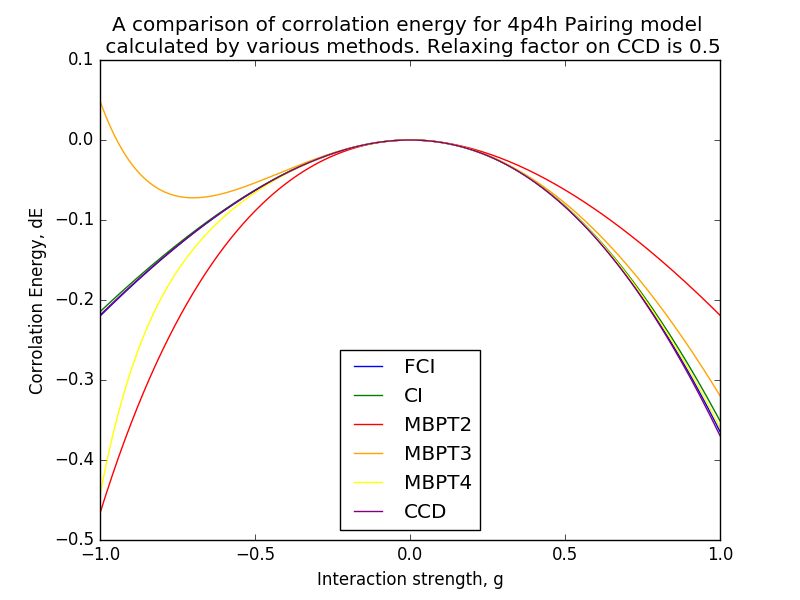
\includegraphics[width=\linewidth]{../Pairing_Model/Results/Figures/Pairing4p4h_CompareDE_AllMethods.png}
				\caption{Comparing }
				\label{Results4}
			\end{figure}

			\begin{figure}
				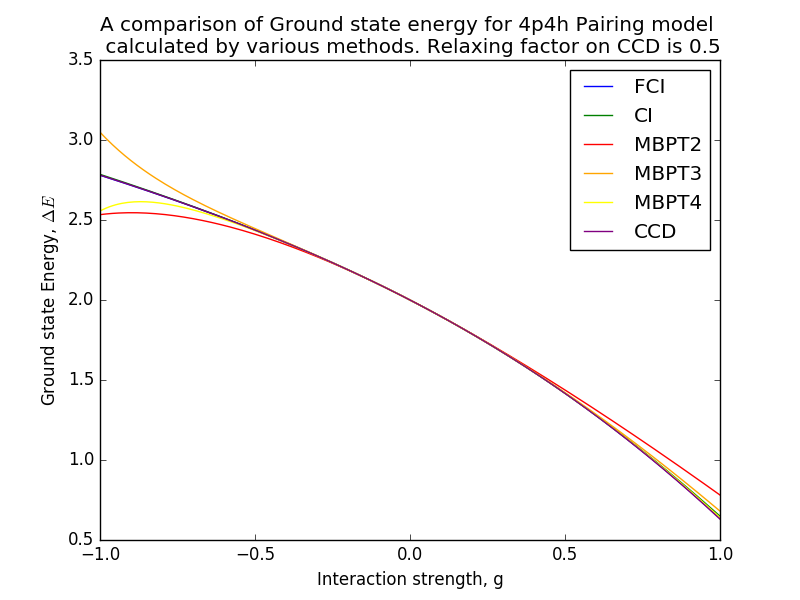
\includegraphics[width=\linewidth]{../Pairing_Model/Results/Figures/Pairing4p4h_CompareE_AllMethods.png}
				\caption{}
				\label{Results5}
			\end{figure}

		\end{subsection}


	\end{section}

\end{chapter}

\begin{chapter}{Conclusion and future prospects}
	
\end{chapter}


\medskip


\begin{thebibliography}{9}

	\bibitem{Baardsen}
	Gustav Baardsen
	\textit{Coupled-cluster theory for infinite matter} 2014

	\bibitem{Audun}
	Audun Skau Hansen
	\textit{Coupled Cluster studies of infinite systems,} Master thesis, University of Oslo, 2015

	\bibitem{ShavittAndBartlett}
	Isaiah Shavitt and Rodney J. Bartlett
	\textit{Many-Body Methods in Chemistry and Physics} 2009

	\bibitem{Szabo}
	Attila Szabo and Neil S. Ostlund
	\textit{Modern Quantum Chemistry. Introduction to Advanced Electronic Structure Theory} 1982

	\bibitem{Griffiths}
	David J. Griffiths
	\textit{Introduction to Quantum Mechanics} Second edition 2005

	\bibitem{Sakurai}
	J.J. Sakurai
	\textit{Modern Quantum Mechanics} Revised Edition 1993

	\bibitem{Hjorth-Jensen2016}
	Morten Hjorth-Jensen, Maria Paola Lombardo and Ubiraja van Kolck
	\textit{An Advanced Course in Computational Nuclear Physics} 2016

	\bibitem{Raimes}
	Stanley Raimes
	\textit{Many-Electron Theory} 1972

	\bibitem{Susskind2014}
	Leonard Susskind and Art Friedman
	\textit{Quantum Mechanics, The Theoretical Minimum} 2014

	\bibitem{Crawford}
	T. Daniel Crawford and Henry F. Schaefer III
	\textit{An Introduction to Coupled Cluster Theory for Computational Chemists} 

	\bibitem{Day1967} 
	B. D. Day
	\textit{Rev. Mod. Phys.,}
	39:719, 1967.

	\bibitem{Thompson1977}
	D. R. Thompson, M. Lemere and Y.C. Tang.
	\textit{Nucl. Phys. A,} 286:53 1977.

	\bibitem{Shepherd2012}
	J. J. Shepherd, A. Grüneis, G.H. Booth, G. Kresse and A. Alavi 
	\textit{Phys. Rev. B,} 86:035111, 2012.

	\bibitem{Shepherd2013}
	J.J. Shepherd and A. Grüneis
	\textit{Phys. Rev. Lett.,} 110:226401, 2013.

	\bibitem{Drummond2008}
	N. D. Drummond, R. J. Needs, A. Sorouri and W. M. C. Foulkes
	\textit{Phys. Rev. B,} 78:125106

	\bibitem{Fraser et al}
	L. M. Fraser, W. M. C. Foulkes, G. Rajagopal, R. J. Needs, S.D. Kenny and A. J. Williamson
	\textit{Phys. Rev. B,} 53:1814, 1996

	\bibitem{Ewald}
	P.P. Ewald. Die berechnung optischer und elektrostatischer gitterpotentiale. 
	\textit{Annalen der Physik,} 369(3), 1921. ISSN 1521-3889. doi: 10.1002/andp.19213690304

	\bibitem{Langtangen}
	Hans Petter Langtangen
	\textit{A Primer on Scientific Programming with Python} Scond Edition, Springer 2011

	\bibitem{NumericalRecipes}
	William H. Press, Saul A. Teukolsky, William T. Vetterling, Brian P. Flannery
	\textit{Numerical Recipes, The Art of Scientific Computing} Third Edition, Cambridge 2007

	\bibitem{MHJFCI}
	Morten Hjorth-Jensen
	\textit{Nuclear Shell Model, Nuclear Talent course 2} 
	URL (14. july, 2016): http://nucleartalent.github.io/Course2ManyBodyMethods/doc/pub/fci/pdf/fci-print.pdf

	\bibitem{MHJonline}
	Carlo Barbieri, Wim Dickhoff, Gaute Hagen, Morten Hjorth-Jensen, Artur Polls
	\textit{Many-body Methods for Nuclear Physics, Nuclear Talent course 2} 
	URL: \textit{http://nucleartalent.github.io/Course2ManyBodyMethods/doc/web/course.html}

	\bibitem{WholmenGithub}
	Fredrik Wilhelm Holmen
	\textit{https://github.com/wholmen/Master} 

	\bibitem{Armadillo}
	Conrad Sanderson. Armadillo: An open source c++ linear algebra library for fast prototyping and computationally intensive experiments, 2010.
	URL: \textit{http://arma.sourceforge.net/docs.html}.

\end{thebibliography}


\end{document}